\documentclass{article}

\usepackage{datetime}
\usepackage[nottoc]{tocbibind}
\usepackage{amssymb}
\usepackage{amsmath}
\usepackage[final]{neurips_2025}
\usepackage{booktabs}
\usepackage{tabularx}
\usepackage[edges]{forest}
\usepackage{pifont}
\usepackage{multirow}
\usepackage{hyperref}
\usepackage[dvipsnames]{xcolor}
\hypersetup{ % 
    colorlinks=true,
    linkcolor=RoyalPurple,
    citecolor=RoyalPurple,
    filecolor=RoyalPurple,
    urlcolor=RoyalPurple,
}
\usepackage{graphicx}
\usepackage{tikz}
\usepackage{adjustbox}
\usepackage{wrapfig}
\usetikzlibrary{shapes.geometric, arrows.meta, positioning, fit, backgrounds, calc}
%\usepackage[square,numbers]{natbib}
\bibliographystyle{abbrvnat}

\usepackage{ragged2e}
\usepackage{array}

\title{Generative Models for \\ Protein-Protein Interaction Prediction}
\author{
  Paul Francis Jarabek Moore \\
  Department of Computer Science \\
  Western University \\
  \texttt{pmoore44@uwo.ca}
}

\newcolumntype{Y}{>{\centering\arraybackslash}X}
\newcolumntype{Z}{>{\raggedleft\arraybackslash}X}

\tikzset{
  data_class_a/.style={circle, draw=blue!80, fill=blue!20, inner sep=2pt},
  data_class_b/.style={rectangle, draw=red!80, fill=red!20, inner sep=2.5pt},
  data_class_none/.style={circle, draw=gray!80, fill=gray!20, inner sep=2pt},
  boundary/.style={thick, dashed, gray!80},
  axis_style/.style={->, thick, black!70},
  label_style/.style={},
  main_box/.style={draw=black, dashed, inner sep=0.7cm, fill=gray!5, rounded corners=3mm},
  encoder/.style={trapezium, draw=blue!80, fill=blue!20, shape border rotate=270,inner sep = 5pt, rounded corners=1mm, minimum width=3cm, trapezium angle=85, trapezium stretches=true},
decoder/.style={trapezium, draw=red!80, fill=red!20, shape border rotate=90,inner sep = 5pt, rounded corners=1mm, minimum width=3cm, trapezium angle=85, trapezium stretches=true},
  vae_data/.style={rectangle, draw=orange!80, fill=orange!20, inner sep=5pt, rounded corners=1mm, minimum height=3cm},
  latent_space/.style={rectangle, draw=green!80, fill=green!20, inner sep=7pt, rounded corners=1mm},
  parameters/.style={rectangle, draw=blue!80, fill=blue!20, inner sep=7pt, rounded corners=1mm},
  op_block/.style={rectangle, draw=orange!80, fill=orange!20, inner sep=5pt, rounded corners=1mm, minimum width=2.5cm, font=\small},
  input_node/.style={font=\large\bfseries},
  arrow/.style={->, thick, black!70, >=Stealth},
neuron_blue/.style={circle, draw=blue!80, fill=blue!20, minimum size=1cm},
  neuron_green/.style={circle, draw=green!80, fill=green!20, minimum size=1cm},
  neuron_yellow/.style={circle, draw=orange!80, fill=orange!20, minimum size=1cm},
  neuron_red/.style={circle, draw=red!80, fill=red!20, minimum size=1cm},
  connect/.style={-, thick, black!70},
var_bar/.style={rectangle, draw=violet!60!black, fill=violet!20, rounded corners=2mm, thick, minimum width=0.8cm},
  output_box/.style={rectangle, draw=violet!60!black, fill=violet!20, rounded corners=2mm, thick, minimum size=1cm},
  arrow/.style={->, thick, black!60, >=Stealth},
  connect/.style={-, black!40, thin},
  label_text/.style={font=\small\bfseries},
  sub_label/.style={font=\Large},
  process_block/.style={rectangle, draw=orange!80!black, fill=orange!20, rounded corners=2mm, thick, minimum width=2.5cm, align=center, font=\small\bfseries\sffamily},
  plm_block/.style={rectangle, draw=blue!80!black, fill=blue!20, rounded corners=2mm, thick, minimum width=2.5cm, align=center, font=\bfseries\sffamily},
  classifier_block/.style={rectangle, draw=red!80!black, fill=red!20, rounded corners=2mm, thick, minimum width=2.5cm, align=center, font=\bfseries\sffamily}
}


\pgfdeclarelayer{boxlayer}
\pgfdeclarelayer{barlayer}
\pgfsetlayers{boxlayer,barlayer, background, main}

\DeclareMathOperator*{\argmin}{arg\,min}

\begin{document}

% Title Page
\maketitle
% Abstract

\begin{abstract}
Protein-Protein interactions (PPIs) lie at the centre of many biological processes. Understanding and predicting these interactions is crucial in drug discovery, as experimental methods are often slow and expensive. Computational techniques have been in development for decades, but recent developments in deep learning have revolutionized PPI Prediction. This paper brings informed non-experts up to speed on the current developments in protein-protein interaction prediction following the deep learning revolution. It provides an in-depth background of relevant topics in machine learning and bioinformatics. Various approaches are reviewed, including methods that leverage sequence, structure, and network information, with an emphasis on generative models. These models include variational autoencoders, transformers, generative adversarial networks, and diffusion models.
\end{abstract}

% Table of Contents
%\tableofcontents
%\newpage

% Introduction
\section{Introduction}
Proteins are essential macromolecules in all living organisms, playing a critical role in the structure, function, and regulation of the body's cells, tissues, and organs. These complex molecules are comprised of long chains of amino acids, which link together and fold into a unique, specific three-dimensional structure. The sequence and subsequent shape are crucial for determining the protein's particular function. Common protein roles include acting as enzymes to catalyze biochemical reactions (like digestion), providing structural support, enabling movement, serving as messengers, and protecting the body as antibodies \citep{reece2011campbell}.

Protein-protein interactions (PPIs) occur when physical contact is established between two or more proteins. PPIs facilitate chemical reactions, the formation of complex machineries, and signal pathways between cells \citep{morris_uncovering_2022}. Each of these is necessary for the essential functions of proteins. Consequently, PPIs can be targets for both diseases and drugs. Accurately predicting these interactions can accelerate the process of designing drugs by allowing cost-effective filtering of potential interactions with a target protein. Traditionally, PPIs are discovered using experimental techniques in a lab, using techniques like yeast 2 hybrid (Y2H) or co-immunoprecipitation (Co-IP). These methods are expensive and time-consuming, and sometimes inaccurate \citep{ding_computational_2018}. For example, Co-IP can take multiple days \citep{tang_analysis_2018}, and Y2H has high throughput \citep{bruckner_yeast_2009}, but has been known to yield results with high false positive rates \citep{vidalain_increasing_2004}. 

There are three categories of PPI detection methods: \textit{in vitro}, \textit{in vivo}, and \textit{in silico}. \textit{In vitro}, the experiment is performed in a controlled environment, outside the organism. \textit{In vivo}, the experiment is performed on the organism. The methods mentioned above belong to these two categories and are typically more expensive than \textit{in silico}, where the experiment is performed in a digital simulation \citep{rao_protein-protein_2014}. \textit{In silico} techniques are particularly attractive with the recent advances in deep learning, allowing unprecedented performance on a variety of problems in bioinformatics, including PPI prediction \citep{zhang_revolutionizing_2024, guo_diffusion_2024}.

Computational (\textit{in silico}) methods for PPI prediction has been an area of interest for decades \citep{dandekar_conservation_1998}. Starting with simple homology searches, and eventually making use of primary (amino acid sequence), secondary (local 3D structures), and tertiary structure (the entire 3D structure) of the proteins. As the field of machine learning advanced, so did PPI prediction techniques by leveraging the new power granted by increasingly sophisticated models.

The field of machine learning (ML) has undergone an unprecedented growth in recent years, primarily fueled by three factors: the availability of massive datasets (Big Data), a dramatic increase in computational power, and algorithmic breakthroughs (notably in deep learning with the rise of deep neural networks). This synergistic combination has enabled ML models to achieve near-human (and sometimes superhuman) performance in complex tasks like image recognition \citep{archana_deep_2024} and natural language processing \citep{qin2025largelanguagemodelsmeet}.

Recently, the most advanced models are generative models, a revolutionary subclass of machine learning that focuses on learning the complex underlying data distribution to create entirely novel outputs rather than just classifying or predicting existing ones. For data features \(x\) and classification labels \(y\), generative models learn the distribution \(p(x)\) rather than the conditional probability \(p(y|x)\), depicted in Figure \ref{visual-abstract}. Models like generative adversarial networks \citep[GANs;][]{goodfellow2014generative}, variational autoencoders \citep[VAE;][]{kingma_vae_2013}, large language models \citep[LLMs;][]{naveed_llm_2025}, and diffusion models \citep{sohl-dickstein_deep_nodate} have demonstrated remarkable ability to synthesize realistic images, text, and biological structures \citep{ramesh2021zeroshottexttoimagegeneration, radford_improving_2018, abramson_accurate_2024}. In the field of protein-protein interaction (PPI) prediction, generative models are excellent at understanding the hidden features of protein sequences and structures, facilitating state-of-the-art accuracy of predictions.

% FIGURE 1
\begin{figure}
  
  \centering
  \resizebox{\textwidth}{!}{
    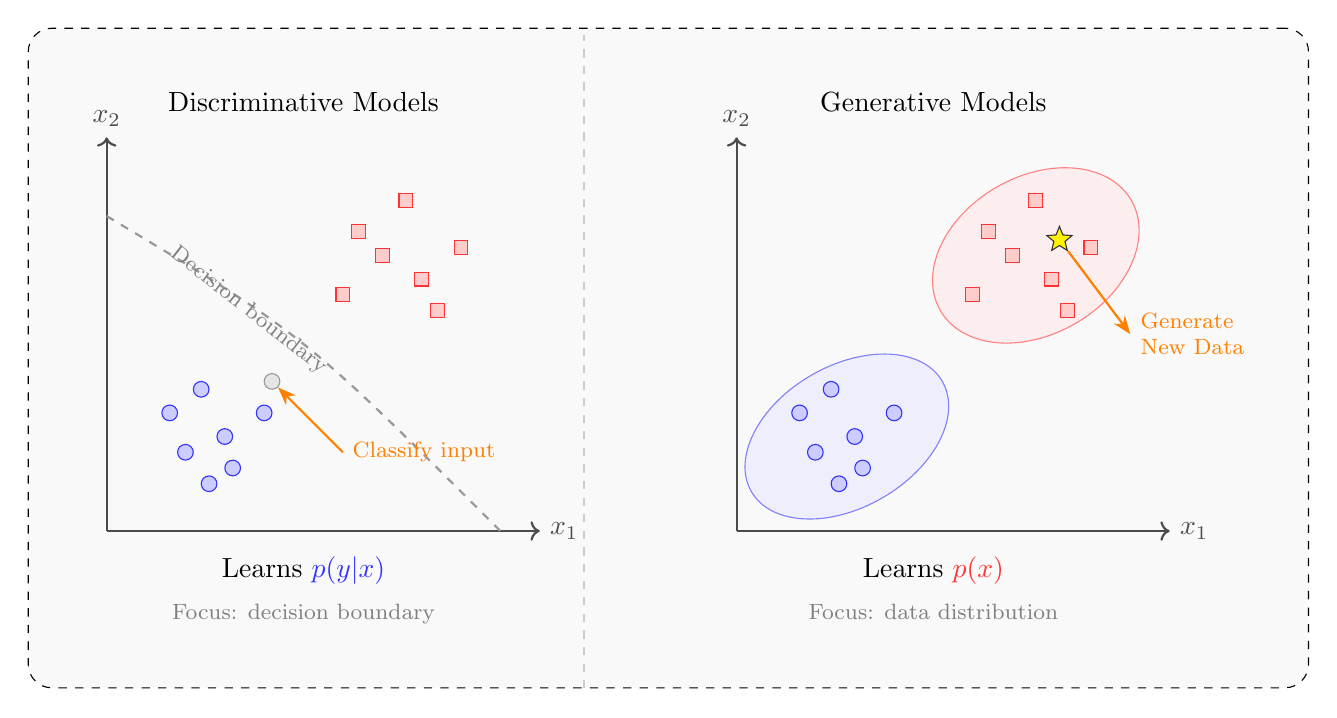
\begin{tikzpicture}[]

      

      \begin{scope}[local bounding box=discriminative]
        % Title
        \node[label_style, anchor=south] at (2.5, 5.2) {Discriminative Models};
        \node[anchor=north] at (2.5, -0.2) {Learns \textcolor{blue!80}{$p(y|x)$}};
        \node[anchor=north, text=gray, font=\footnotesize] at (2.5, -0.8) {Focus: decision boundary};

        % Axes
        \draw[axis_style] (0,0) -- (5.5,0) node[right] {$x_1$};
        \draw[axis_style] (0,0) -- (0,5) node[above] {$x_2$};

        \foreach \point in {(1,1), (1.5,1.2), (1.2,1.8), (0.8,1.5), (1.6, 0.8), (2, 1.5), (1.3, 0.6)} {
          \node[data_class_a] at \point {};
        }

        \foreach \point in {(3.5,3.5), (4,3.2), (3.2,3.8), (3.8,4.2), (4.2, 2.8), (3, 3), (4.5, 3.6)} {
          \node[data_class_b] at \point {};
        }

        \draw[boundary] (0, 4) .. controls (2.5, 2.5) .. (5, 0);
        \node[text=gray, rotate=-38, font=\footnotesize] at (1.8, 2.8) {Decision boundary};
    
        \node[data_class_none] (input) at (2.1, 1.9) {};
        \draw[arrow, orange] (3, 1) -- (input);
        \node[text=orange, font=\footnotesize, anchor=west] at (3, 1) {Classify input};

      \end{scope}

      \begin{scope}[xshift=8cm, local bounding box=generative]
        % Title
        \node[label_style, anchor=south] at (2.5, 5.2) {Generative Models};
        \node[anchor=north] at (2.5, -0.2) {Learns \textcolor{red!80}{$p(x)$}};
        \node[anchor=north, text=gray, font=\footnotesize] at (2.5, -0.8) {Focus: data distribution};

        % Axes
        \draw[axis_style] (0,0) -- (5.5,0) node[right] {$x_1$};
        \draw[axis_style] (0,0) -- (0,5) node[above] {$x_2$};

        \filldraw[draw=blue!50, fill=blue!10, fill opacity=0.5, rotate around={30:(1.4, 1.2)}] (1.4, 1.2) ellipse (1.4 and 0.9);
        \filldraw[draw=red!50, fill=red!10, fill opacity=0.5, rotate around={30:(3.8, 3.5)}] (3.8, 3.5) ellipse (1.4 and 1.0);

        \foreach \point in {(1,1), (1.5,1.2), (1.2,1.8), (0.8,1.5), (1.6, 0.8), (2, 1.5), (1.3, 0.6)} {
          \node[data_class_a] at \point {};
        }

        \foreach \point in {(3.5,3.5), (4,3.2), (3.2,3.8), (3.8,4.2), (4.2, 2.8), (3, 3), (4.5, 3.6)} {
          \node[data_class_b] at \point {};
        }
    
        \node[star, star points=5, star point ratio=2.25, draw=black!80, fill=yellow, inner sep=1.5pt] (new_sample) at (4.1, 3.7) {};
        \draw[arrow, orange] (new_sample) -- (5, 2.5) node[right, text=orange, font=\footnotesize, align=left] {Generate\\New Data};

      \end{scope}

      \draw[dashed, thick, gray!40] (0.5\textwidth, -2) -- (0.5\textwidth, 6.3);

      \begin{scope}[on background layer]
        \node[main_box, fit=(discriminative.south west) (generative.north east) (discriminative.north east) (generative.south west)] (big_box) {};
      \end{scope}  
    \end{tikzpicture}
  }

\caption{Generative vs. discriminative models.}
\label{visual-abstract}
\end{figure}

Previous work has surveyed multiple different areas of computational PPI prediction. \citet{rao_protein-protein_2014} provided a broad but superficial review of all methods at the time (over a decade ago), including \textit{in vitro} and \textit{in vivo} methods. \citet{ding_computational_2018} classified the computational methods by which features of the proteins are used for prediction (sequence, structure, network, genome, function). \citet{charih_sequence-based_2025} covered only sequence-based approaches with a focus on methods that use the transformer architecture, and provided a review of real-world applications and deployments of such models. \citet{kiouri_structure-based_2025} covered only structure-based approaches, with a focus on modern deep learning (DL) models. \citet{zhang_revolutionizing_2024} reviews advances in both structure prediction and interaction prediction. \citet{taha_protein-protein_2025} provides a deeper background of the architectures being used and empirical testing for many models. However, none cover the application of generative models for predicting PPIs in-depth. This current work fills that research gap by first providing some background information on recent developments in generative AI, then a brief history of PPI prediction techniques using discriminative models like support vector machines \citep[SVM;][]{cortes_support-vector_1995} and convolutional neural networks \citep[CNN;][]{lecun_backpropagation_1989}, among others. Finally, we describe the current state of the field, analyzing the most recent contributions to the field, including models that leverage the pivotal transformer architecture or the more recent discovery of diffusion models.

% Background
\section{Background}
This section provides all the necessary background information required to properly get up to speed on the current state-of-the-art in PPI prediction. We begin with proteins and PPIs, then datasets, and historical methods for PPI prediction. Next, we provide background on fundamental models in machine learning like neural networks \citep[NNs;][]{rosenblatt_perceptron_1958}, autoencoders, convolutional neural networks \citep[CNNs;][]{lecun_backpropagation_1989}, recurrent neural networks (RNNs), long short-term memory \citep[LSTMs;][]{lstm}. Then, word embedding models are discussed as well as their transferability to proteins. Finally, we discuss generative models like variational autoencoders \citep[VAEs;][]{kingma_vae_2013}, generative adversarial networks \citep[GANs;][]{goodfellow2014generative}, transformers \citep{vaswani_attention_2017}, and diffusion models \citep{sohl-dickstein_deep_nodate}.

\subsection{Proteins}

\begin{wraptable}[27]{r}{7cm}
    \caption{The 22 amino acids used to form proteins, and their symbols. ``*'' denotes specialized amino acids found in specific organisms or enzymes.}
    \label{AA}
    \begin{tabularx}{7cm}{lcY}
      \toprule
        \textbf{Amino Acid} & \textbf{3-Letter Code} & \textbf{1-Letter Symbol} \\ \midrule
        Alanine & Ala & A \\ 
        Arginine & Arg & R \\ 
        Asparagine & Asn & N \\
        Aspartic Acid & Asp & D \\
        Cysteine & Cys & C \\ 
        Glutamic Acid & Glu & E \\
        Glutamine & Gln & Q \\ 
        Glycine & Gly & G \\ 
        Histidine & His & H \\
        Isoleucine & Ile & I \\
        Leucine & Leu & L \\ 
        Methionine & Met & M \\ 
        Phenylalanine & Phe & F \\ 
        Proline & Pro & P \\ 
        Selenocysteine* & Sec & U \\ 
        Serine & Ser & S \\ 
        Threonine & Thr & T \\
        Tryptophan & Trp & W \\
        Tyrosine & Tyr & Y \\
        Valine & Val & V \\
        Pyrrolysine* & Pyl & O \\\bottomrule 
      \end{tabularx}
\end{wraptable}

Proteins are the building blocks of life, serving as catalysts for countless crucial chemical reactions that occur in organisms, structurally support cells and tissues, hormones, enzymes, etc. \citep{lapelusa_physiology_2022}. At the most basic level, proteins are composed of a chain of amino acids. Amino acids are molecules called organic compounds that are part of both the amino and carboxylic acid functional groups \citep{lehninger_biochemistry_1970}. Of the hundreds of amino acids, only 20 common amino acids are used to create proteins, and an additional 2 are found in specific organisms or enzymes. Each of these 22 amino acids is assigned a single letter code (Table \ref{AA}). 

Amino acids link to each other through peptide bonds and other molecular interactions, imposing various forces on the protein. These interactions result in the ``folding'' of the protein into a particular shape. This shape can vary slightly based on the environment and interactions with other proteins \citep{alberts_shape_2002}. 

\subsection{Protein Interactions}
Almost no proteins work in isolation; they need some other compound to interact with as a catalyst, or form a signal pathway, or complete some other function \citep{morris_uncovering_2022}. Inside a cell, proteins will collide with ligands (small molecules that bind to proteins), peptides (small chains of amino acids), or even other proteins. If the orientation of these compounds is correct, they will chemically bond to one another. These interactions are classified into 4 categories: transient, obligate, homo-oligomeric, and hetero-oligomeric. Transient interactions form and dissociate quickly. The interaction partners, therefore, exist in isolation most of the time. Obligate interactions form stable complexes between two compounds that rarely exist in isolation. Homo-oligomeric interactions occur between proteins and identical copies of themselves. They can form complexes with multiple copies at a time, not just two. Finally, hetero-oligomeric interactions form complexes with non-identical proteins. 

Determining whether two given proteins will interact with each other at all is a fundamental problem in biology that has been extensively researched. Methods for solving this problem have been historically confined to a lab \cite{akbarzadeh_studying_2024}, but in recent years, with the advances in ML, computational methods have been gaining traction.

Computational methods for PPI prediction train ML models on large protein interaction and protein datasets (see Section \ref{Datasets}) in order to accurately determine, when given two proteins (or a network of protein interactions), whether or not they will interact. Other problems in bioinformatics take a similar approach, such as binding affinity prediction \citep{stephenson_recent_2025}, where it is predicted how strong an interaction is between a protein and a ligand (typically), or interaction site prediction \citep{aumentado-armstrong_algorithmic_2015}, where, given two proteins, the physical location of the interaction is predicted.

When predicting PPIs, there are three data sources to choose from: sequence, structure, or network. Sequence-based PPI prediction uses only the amino acid sequences of both proteins to determine whether or not they interact. Using only the sequence information is more efficient than using structural or network information, but is more challenging since the structure of a protein is a defining factor of its behaviour. 

Structural information intrinsically includes sequence information, as it contains a 3D coordinate of each amino acid in the sequence. Avoiding the need to learn the structure of the protein from the sequence makes the problem easier, but may not be as applicable since structural information is more scarce and expensive to obtain than sequence. There has been some work to make standalone models for predicting the structure (AlphaFold \citep{abramson_accurate_2024}), which could make structure-based approaches more viable.

Finally, one can predict PPIs based on known PPIs in the same interactome. This method is generally not applicable, as it learns nothing about the proteins themselves, and is not generalizable to interaction networks it did not see in training. This can be addressed by incorporating sequence, structure, or both into the prediction, but there will still be a tendency to learn the topology of the network rather than the intricacies of the proteins.

\subsection{History}
For computational PPI prediction, historically, features of protein sequences and structures were extracted via engineered methods \citep{charih_sequence-based_2025}. Conjoint triad (CT) summarizes a protein sequence by grouping the 20 standard amino acids into seven classes based on their physicochemical properties and then counting the frequency of all possible $7\times7\times7=27$ triad combinations within the sequence \citep{shen_predicting_2007}. Autocovariance (AC) captures the correlation or dependency between amino acids at a specific distance (lag) apart along the protein sequence based on their physicochemical properties, averaging this covariance over the entire sequence \citep{guo_using_2008}. Amino acid composition (AAC) represents proteins as a fixed-length vector containing the frequency of each amino acid in the sequence. Pseudo amino acid composition (PseAAC) extends AAC to include some sequence order information by measuring the correlation of physicochemical properties of amino acids up to a certain $\lambda$ apart \citep{chou_pseaac_2001}. Position-specific scoring matrix (PSSM) is generated by PSI-BLAST \citep{altschul_gapped_1997} from multiple sequence alignments of homologous proteins and represents the conservation probability of each amino acid. These methods encode some important information about the sequences, and importantly, output a fixed-length representation of proteins regardless of their length, but are ultimately incapable of sufficiently capturing the complexity of biological systems individually. Such feature extraction methods were commonly used directly as input into a classical discriminative model. \citet{shen_predicting_2007} and \citet{guo_using_2008} both used SVMs as their classification method, with CT and AC as the feature extraction, respectively.

Later methods use representation learning, where an algorithm automatically discovers, or extracts, critical features from raw data. Methods like autoencoders, word embeddings, and deep neural networks (DNNs) achieve this.

\subsection{Datasets}\label{Datasets}
% TABLE 1
\begin{table}
  \caption{PPI Databases, the number of interactions they contain, and the number of unique sequences. Negatome 2.0 \citep{blohm_negatome_2013} and \citet{bernett_cracking_2024} did not disclose the exact number of proteins.}
  \label{ppi-databases}
  \centering
  \begin{tabularx}{\textwidth}{l X r r}
    \toprule
    \textbf{Database} & \textbf{Reference} & \textbf{Interactions} & \textbf{Sequences}\\
    \midrule
    BioGRID & \citep{oughtred_biogrid_2021} & 2,911,104 & 91,289 \\
    IntAct & \citep{orchard_mintact_2013} & 1,726,205 & 145,895 \\
    STRING & \citep{szklarczyk_string_2022}  & 27,541,372,832 & 59,309,604 \\
    MINT & \citep{licata_mint_2011}  & 137,544 & 27,555 \\
    Mentha & \citep{calderone_mentha_2013}  & 741,337 & 90,905\\
    Negatome Database 2.0 & \citep{blohm_negatome_2013}  & 6,532 & \(\approx\) 1,900\\
    Bernett Gold Standard & \citep{bernett_cracking_2024}  & 274,500 & \(\approx\) 14,077 \\
    \bottomrule
  \end{tabularx}
\end{table}

Labeled datasets of interacting pairs of proteins are required to evaluate the accuracy of PPI prediction models. Databases like BioGRID, IntAct, and STRING provide millions of interacting pairs of proteins, but no non-interacting pairs. Such negative datasets are critical to the training of prediction algorithms \citep{ben-hur_choosing_2006}. There are negative datasets like Negatome DB 2.0 \citep{blohm_negatome_2013} which contains only 6,532 examples in contrast with the massive sets of positive examples like BioGRID, IntAct, or STRING which contain millions (see Table \ref{ppi-databases}).

For a generative model to learn the language of proteins and be able to properly extract information from individual proteins, the labeled interaction data is not necessary. Furthermore, databases like STRING \citep{szklarczyk_string_2022} do not always include information on the tertiary structure of the proteins. Therefore, separate databases, which contain individual protein data like primary structure (UniProt \citep{consortium_uniprot_2024}, RefSeq \citep{goldfarb_ncbi_2024}) or tertiary structure (PDB \citep{berman_protein_2000}, AlphaFold DB \citep{bertoni_alphafold_2025}) are used. Some common protein databases are presented in Table \ref{protein-databases}.

A common issue among published PPI prediction methods is data leakage from randomly splitting such datasets into train/test partitions \citep{bernett_cracking_2024}. \citet{bernett_cracking_2024} conducted a study evaluating many of the state-of-the-art models on datasets specifically crafted to determine whether the models are truly learning the underlying patterns of protein-protein interaction, or if they are relying on sequence similarity or node degree information shortcuts (hub proteins). They concluded that such shortcuts are entirely responsible for the high accuracy in the literature. As a result of these findings, \citet{bernett_cracking_2024} created a new gold standard dataset for evaluating sequence-based PPI prediction models that ensures the absence of data leakage and released it publicly.

% TABLE 2
\begin{table}
  \centering
\caption{Protein databases, the number of individual proteins they contain, and the dominant source of proteins.}
  \label{protein-databases}
  \begin{tabularx}{\textwidth}{l X r r}
    \toprule
    \textbf{Database} & \textbf{Reference} & \textbf{Proteins} & \textbf{Most represented}\\
    \midrule
    UniProt & \citep{consortium_uniprot_2024}  & 199,579,900 & Homo sapiens \\ 
    PDB (Experimental) & \citep{berman_protein_2000}  & 246,045 & Homo sapiens \\ 
    AlphaFold DB & \citep{bertoni_alphafold_2025}  & 241,070,489 & Glycine max \\ 
    RefSeq & \citep{goldfarb_ncbi_2024}  & 427,129,536 & Bacteria \\ 
    \bottomrule
  \end{tabularx}
\end{table}



%TODO Find papers for each of these sections, use ones from the paragraph below, and find more examples.
%TODO Summarize each paper
%TODO Explain each model type similar to the generative models section
\subsection{Neural Networks}\label{NNsec}

\begin{figure}[htbp]
  \centering 
  \begin{adjustbox}{width=\textwidth}
    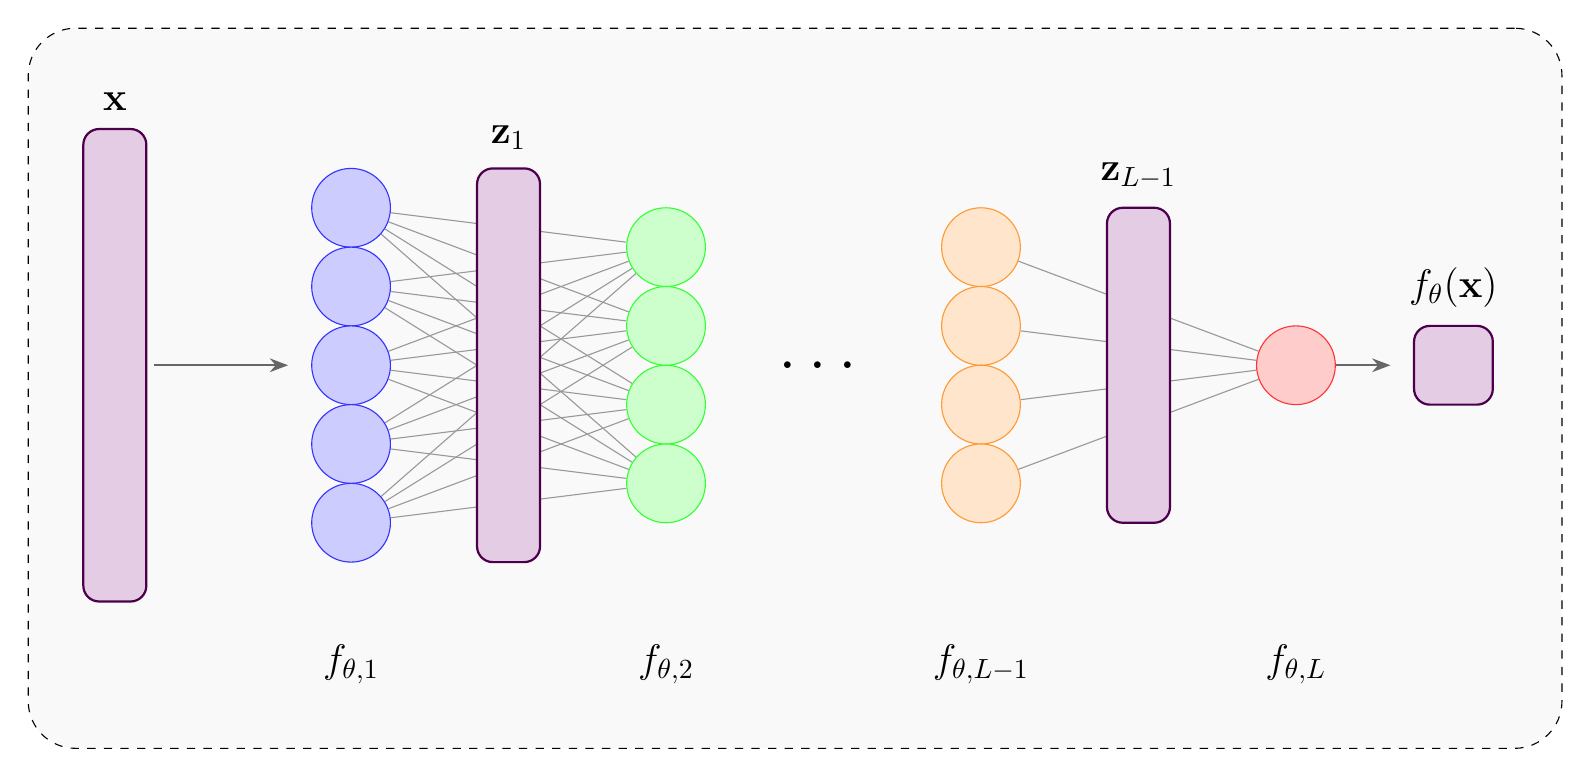
\begin{tikzpicture}
      
      % --- Define Layers ---
      \pgfdeclarelayer{background}
      \pgfdeclarelayer{barlayer}
      \pgfdeclarelayer{boxlayer}
      \pgfsetlayers{boxlayer,background,barlayer,main}

      % Define a scope to capture the bounding box
      \begin{scope}[local bounding box=nn_content]

        % --- Geometry Definitions (Significantly Wider) ---
        \def\xInput{0}
        \def\xLOne{3}     % Increased spacing
        \def\xZOne{5}
        \def\xLTwo{7}
        \def\xDots{9}
        \def\xLThree{11}
        \def\xZLast{13}
        \def\xOutNode{15}
        \def\xFinal{17}
        
        \def\yLabel{-3.8} % Baseline for bottom labels

        % --- Input x ---
        \node[var_bar, minimum height=6cm] (input_x) at (\xInput, 0) {};
        \node[label_text, font=\Large, above=0.1cm of input_x] {$\mathbf{x}$};
        \draw[arrow] (\xInput+0.5, 0) -- (\xLOne-0.8, 0);

        % --- Layer 1 (Blue): 5 Nodes (Original Count) ---
        \foreach \i in {1,...,5} {
          \node[neuron_blue] (L1-\i) at (\xLOne, {2 - (\i-1)}) {};
        }
        \node[sub_label] at (\xLOne, \yLabel) {$f_{\theta,1}$};

        % --- Layer 2 (Green): 4 Nodes (Original Count) ---
        \foreach \i in {1,...,4} {
          \node[neuron_green] (L2-\i) at (\xLTwo, {1.5 - (\i-1)}) {};
        }
        \node[sub_label] at (\xLTwo, \yLabel) {$f_{\theta,2}$};

        % --- Connections L1 -> L2 ---
        \begin{pgfonlayer}{background}
          \foreach \i in {1,...,5} {
            \foreach \j in {1,...,4} {
              \draw[connect] (L1-\i) -- (L2-\j);
            }
          }
        \end{pgfonlayer}

        % --- Bar z1 ---
        \begin{pgfonlayer}{barlayer}
          \node[var_bar, minimum height=5cm] (z1) at (\xZOne, 0) {};
        \end{pgfonlayer}
        \node[label_text, font=\Large, above=0.1cm of z1] {$\mathbf{z}_1$};

        % --- Ellipsis ---
        \node[font=\Huge] at (\xDots, 0) {$\dots$};

        % --- Layer L-1 (Yellow): 4 Nodes (Original Count) ---
        \foreach \i in {1,...,4} {
          \node[neuron_yellow] (L3-\i) at (\xLThree, {1.5 - (\i-1)}) {};
        }
        \node[sub_label] at (\xLThree, \yLabel) {$f_{\theta,L-1}$};

        % --- Output Node (Red): 1 Node ---
        \node[neuron_red] (OutNode) at (\xOutNode, 0) {};
        \node[sub_label] at (\xOutNode, \yLabel) {$f_{\theta, L}$};

        % --- Connections L(L-1) -> Output ---
        \begin{pgfonlayer}{background}
          \foreach \i in {1,...,4} {
            \draw[connect] (L3-\i) -- (OutNode);
          }
        \end{pgfonlayer}

        % --- Bar z_(L-1) ---
        \begin{pgfonlayer}{barlayer}
            \node[var_bar, minimum height=4cm] (zLast) at (\xZLast, 0) {};
        \end{pgfonlayer}
        \node[label_text, font=\Large, above=0.1cm of zLast] {$\mathbf{z}_{L-1}$};

        % --- Final Output Box ---
        \draw[arrow] (OutNode) -- (\xFinal-0.8, 0);
        \node[output_box] (final_out) at (\xFinal, 0) {};
        \node[label_text, font=\Large, above=0.1cm of final_out] {$f_\theta(\mathbf{x})$};

      \end{scope}

      % --- Background Box ---
      \begin{pgfonlayer}{boxlayer}
        \node[main_box, rounded corners=6mm, fit=(nn_content)] {};
      \end{pgfonlayer}

    \end{tikzpicture} 
  \end{adjustbox}
  \caption{The general architecture of a neural network with \(L\) layers.}
  \label{NN}
\end{figure}

Most modern machine learning algorithms today are based on the idea of a neural network: a concept originally inspired by the biology of brains. The first of which was pioneered by \citet{rosenblatt_perceptron_1958} with the perceptron, a single-layer neural network. One drawback of the original perceptron was its inability to learn to classify non-linearly separable data. \citet{rumelhart_learning_1986} introduced the backpropagation algorithm, which allowed easy training of multi-layer perceptrons, which could be fitted with non-linear activation functions. This solved the original perceptron's problem, but introduced new issues like vanishing gradient, lack of computational power, and limited data. In recent years, each of these issues has been more or less solved with huge amounts of computational power, data, and algorithmic innovations like the ReLU activation function or dropout. With more computing power, data, and a wider variety of algorithms came DNNs. DNNs are fundamentally based on MLPs, but have a large number of hidden layers.


A DNN \(f_\theta\) can be expressed as a composition of layers \(f_\theta^l:\mathbb{R}^{d_{l-1}}\rightarrow\mathbb{R}^{d_l}\) and non-linear functions \(h:\mathbb{R}\rightarrow\mathbb{R}\) applied component-wise:
\[f_\theta(x) = f_{\theta,L}(h(f_{\theta,L-1}(...(f_{\theta,1}(x))...)))\] 
where \(L\) is the number of layers in the network. Each function/layer \(f_{\theta,l}\) has it`s own set of parameters \(\theta\), which govern the weights \(\mathbf{W}\) and bias \(\mathbf{b}\) of each neuron. For example, a fully connected layer (each neuron takes as input the output of each of the previous layer's neurons, see Figure \ref{NN}):
\[f_{\theta,l}(\mathbf{z}_{l-1}) = \mathbf{W}_l\mathbf{z}_{l-1} + \mathbf{b}_l\]
\[\mathbf{z}_l = h(f_{\theta,l}(\mathbf{z}_{l-1}))\]

Training neural networks is done by minimizing a loss function. Simply put, a loss function measures the distance from the model`s output to the correct value. For example, a common loss function is the mean squared error (MSE) loss:
\[\mathcal{L}(\theta, x, y) = \frac{1}{N}\displaystyle\sum_{i=1}^{N}(f_\theta(x_i) - y_i)^2\] 

The output of the penultimate, or final hidden layer \(\mathbf{z}_{L-1}\) is the internal representation of the input \(x\), which is used for whatever task is required, be it classification or regression.



\subsection{Autoencoders}

Autoencoders learn to compress data into a compressed latent space, then reconstruct the original data with minimal loss (see Figure \ref{AE}). This requires the latent space to preserve the most important features. An autoencoder is comprised of two neural networks: the encoder \(\text{Enc}_\theta : \mathcal{X}\rightarrow \mathbb{R}^K\), and the decoder \(\text{Dec}_\phi : \mathbb{R}^K\rightarrow \mathcal{X}\) where \(\mathcal{X}\) is the set of all possible inputs, and \(K\) is the number of dimensions for the latent vectors.



Both networks are typically trained in tandem, for example, by minimizing the total reconstruction loss 
\[\argmin_{\theta,\phi} \frac{1}{2}\displaystyle\sum_{n=1}^{N}||x_n-\text{Dec}_\phi(\text{Enc}_\theta(x_n))||_2^2\]

While autoencoders work for learning a compressed representation of the input, they are not capable of generating new data. That is, they were not designed to learn the underlying distribution \(p(x)\). Variational autoencoders \citep{kingma_vae_2013} address this issue, and are covered in section \ref{VAE-sec}

\begin{figure}
  
  \centering
  \resizebox{\textwidth}{!}{
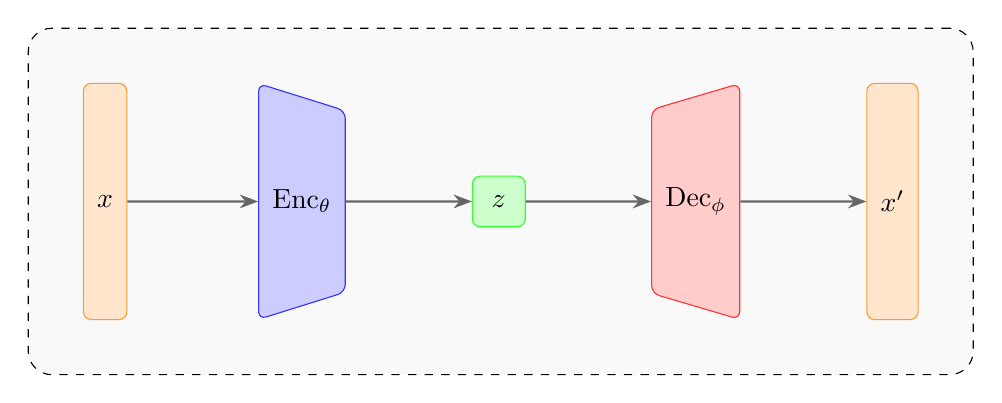
\begin{tikzpicture}
    % Using a scope for the main content with a bounding box name
    \begin{scope}[local bounding box=ae_diagram]
      
      % Nodes defined using the styles from your example and absolute positioning
      \node[vae_data](input) at (0, 0) {\(x\)};
      \node[encoder](encoder) at (2.5,0) {\(\text{Enc}_\theta\)};
      % In a standard AE, this is often just called the bottleneck or latent vector 'z'
      \node[latent_space](bottleneck) at (5,0){\(z\)}; 
      \node[decoder](decoder) at (7.5,0) {\(\text{Dec}_\phi\)};
      \node[vae_data](output) at (10,0) {\(x'\)};

      % Edges using the thick arrow style
      \draw[arrow] (input) -- (encoder);
      \draw[arrow] (encoder) -- (bottleneck);
      \draw[arrow] (bottleneck) -- (decoder);
      \draw[arrow] (decoder) -- (output);
      
    \end{scope}
    
    % Background box fitting the content scope
    \begin{scope}[on background layer]
        \node[main_box, fit=(ae_diagram.north west)(ae_diagram.south east)] (big_box) {};
    \end{scope} 
\end{tikzpicture}
  }
  \caption{The general architecture of an autoencoder, with an encoder parametrized by \(\theta\), latent dimension \(K\), and decoder parametrized by \(\phi\).}
\label{AE}
\end{figure}

In the context of PPI prediction, \citet{sun_sequence-based_2017} is an example of the use of autoencoders. Their model used CT and AC as input for a stacked autoencoder (SAE) to learn features, and added a softmax classifier head for the final output.



\subsection{Convolutional Neural Networks}
CNNs are a class of deep learning models specifically designed to process grid-like data, most notably images. Traditional neural networks struggle with the high dimensionality of such data, but CNNs excel, identifying patterns like edges, textures, and, with enough layers, complex objects. 

A CNN typically consists of three components: convolution, pooling, and classification/regression. The convolutional component uses a kernel matrix that slides across the input, performing some operation (like dot product) at each position. There may be many convolution layers in the network, each serving to detect different features depending on the kernel. The output of the convolution layer for 2D input (like an image), often called the feature map, is defined as 

\[\mathbf{F}^{I\times J}(i,j) = f_{i,j} = \displaystyle\sum_{m=1}^{M}\displaystyle\sum_{n=1}^{N} x_{i+m, j+n}k_{m,n}\]

where \(x_{i+m,j+n}\) is the value of the input matrix \(\mathbf{X}^{I+m\times J+n}\) at position \(i+m,j+n\) and \(k_{m,n}\) is the kernel matrix \(\mathbf{K}^{M\times N}\) at position \(m,n\). Since the feature map is always smaller than the input matrix, the input must be padded if it is required to maintain its original size. For simplicity, we say that

\[\mathbf{F} = \text{conv}(\mathbf{X})\]

Pooling downsamples the output of the convolutional layers in order to reduce computational complexity without compromising any important features of the image \citep{zafar_convolutional_2024}. Pooling works by combining in some way (e.g., average, max, min) segments of the data. Max pooling can be defined as
\[ \mathbf{Y}_{i,j} = max_{m,n \in \mathbf{W}_{i,j}} \mathbf{X}_{m,n} \]

where \(\mathbf{Y}_{i,j}\) is the output after pooling at position \(i,j\), \(\mathbf{W}_{i,j}\) is the set of indicies of the input \(\mathbf{X}\) for the region covered by the pooling window. Finally, the multi-dimensional data can be flattened into a vector and used as input for some NN, which will perform the final classification or regression. As a shorthand, we say 

\[\mathbf{Y} = \text{maxpool}(\mathbf{X})\]

A recent example of a PPI prediction model that utilized CNNs is \citet{chen_multifaceted_2019}`s PIPR. In particular, they pass pre-trained Skip-Gram (based on Word2Vec \cite{mikolov_word2vec_2013}) embeddings into an array of CNNs, and then an array of RNNs. The resulting embeddings from each protein are multiplied element-wise and passed to an MLP for classification. PIPR was also trained on the tasks of binding affinity and interaction type prediction.

\subsection{Word Embeddings}

Natural language processing (NLP) is the field at the intersection of computer science and linguistics. Its primary goal is to enable computers to understand, interpret, generate, or process human language in a useful way. All modern LLMs like OpenAI`s GPT \citep{brown_language_2020} or Google`s Gemini \citep{team2025gemini} are incredibly capable in each of these aspects. 

Static word embedding methods like Word2Vec \citep{mikolov_word2vec_2013} or FastText \citep{bojanowski_fasttext_2016} train on a large corpus to predict context words (words that appear around a given target word). The embeddings are contained in the final learned weight matrix connecting the input layer to the hidden layer. The embedding for each word contains useful semantic information. 

One classic example for how word embeddings work is the \(\text{King}-\text{Man}+\text{Woman}\approx \text{Queen}\) equation \citep{mikolov_word2vec_2013}(Figure \ref{WE}), which demonstrates at least some understanding of each of the words as well as their interaction with one another. This understanding allowed models like Word2Vec to be applied to a variety of problems in linguistics, like part-of-speech (POS) tagging, named entity recognition (NER), or sentiment analysis \citep{sivakumar_review_2020}.

\begin{wrapfigure}[24]{r}{7cm}
  
  \centering
  \resizebox{0.45\textwidth}{!}{
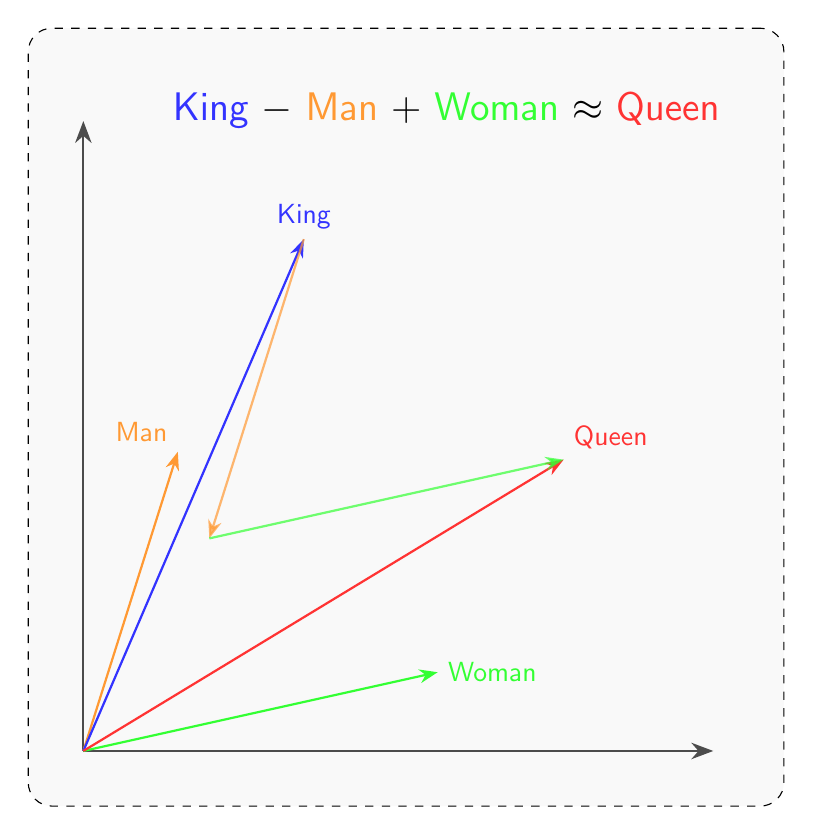
\begin{tikzpicture}[
    >={Stealth[scale=1.2]}, 
    very thick,             
    font=\sffamily          
]
\begin{scope}[local bounding box=box]
    % 1. Define coordinates
    \coordinate (O) at (0,0);
    \coordinate (vecMan) at (1.2, 3.8);
    \coordinate (vecWoman) at (4.5, 1.0);
    \coordinate (vecKing) at (2.8, 6.5);
    \coordinate (vecQueen) at ($(vecKing) - (vecMan) + (vecWoman)$);

    % 2. Draw the Axes
    \draw[axis_style] (O) -- (8,0); % X-axis
    \draw[axis_style] (O) -- (0,8); % Y-axis

    % 3. Draw main vectors from origin using your palette
    \draw[arrow, orange!80] (O) -- (vecMan) node[anchor=south east] {Man};
    \draw[arrow, green!80] (O) -- (vecWoman) node[anchor=west] {Woman};
    \draw[arrow, blue!80] (O) -- (vecKing) node[anchor=south] {King};
    \draw[arrow, red!80] (O) -- (vecQueen) node[anchor=south west] {Queen};

    % 4. Draw the arithmetic path (K - M + W)
    \coordinate (pathPoint1) at ($(vecKing) - (vecMan)$);
    % -Man segment
    \draw[arrow, orange!80, opacity=0.7] (vecKing) -- (pathPoint1);
    % +Woman segment
    \draw[arrow, green!80, opacity=0.7] (pathPoint1) -- (vecQueen);

    % 5. Add the stylized equation at the top
    \node[anchor=north west, font=\sffamily\Large] at (1, 8.5) {
        \textcolor{blue!80}{King} $-$ \textcolor{orange!80}{Man} $+$ \textcolor{green!80}{Woman} $\approx$ \textcolor{red!80}{Queen}
    };
\end{scope}
\begin{scope}[on background layer]
        \node[main_box, fit=(box.south west) (box.north east) (box.north east) (box.south west)] (big_box) {};
      \end{scope} 

\end{tikzpicture}}
  %\resizebox{0.5\textwidth}{!}{
  %  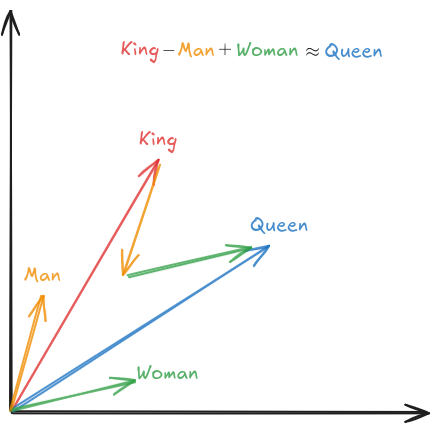
\includegraphics{figs/we.png}
  %}
  \caption{The classic \(\text{King}-\text{Man}+\text{Woman}\approx \text{Queen}\) example \citep{mikolov_word2vec_2013} illustrated.}
\label{WE}
\end{wrapfigure}

One shortcoming of such models is their inability to capture the context of the words. In natural language, the meaning of a word changes depending on the surrounding words in the sentence, so assigning a single, static vector to every instance of a word does not make sense. For example, in the sentences:
\[\text{I ate an \textbf{orange}}\]
\[\text{My car is \textbf{orange}}\]
The word orange has two different meanings. The first is a noun representing the fruit, and the second is used as an adjective for a car. While keeping the deployment cost of such models low (since you only need to compute the embeddings once) is nice, context is important for most aspects of natural language. Thus, more modern embedding models like the LLMs mentioned above, or simpler transformer (see Section \ref{Transformers}) based models like BERT \citep{bert}, T5 \citep{raffel_exploring_2020}, or XLNet \citep{yang_xlnet_2019} capture the context of each instance of a word at the cost of more computational cost as the entire sentence must be used as input each time an embedding is generated. 

A common technique for training a contextual word embedding model is masked language modeling (MLM). MLM is a denoising objective that has the model predict tokens that were randomly masked or corrupted. Essentially, the model learns to ``fill in the blanks''. The output of the final hidden layer \(\mathbf{z}_{L-1}\) (recall Section \ref{NNsec}) can be extracted and used as a contextually rich word embedding.

\subsection{Protein Embeddings}
Clearly, word embeddings are a powerful tool for NLP, and demonstrate that a model can learn the underlying patterns and behaviours of a complex system like a human language. So why not do the same with the ``language'' of the human body?

A protein \(\mathbf{p}\) of length \(N\) can be represented as a vector of amino acids (residues):
\[\mathbf{p} = [a_1, a_2, ..., a_{N-1}, a_N]^\intercal\]
If we consider each amino acid to be a word, and our protein sequence a sentence, then it should be possible to learn representations of proteins in the same way that word embedding models do. Indeed, embedding models based on many word embedding models started appearing. For example, \citet{asgari_continuous_2015} proposed ProtVec based on Word2Vec, ProtBert \citep{brandes_proteinbert_2022} based on BERT, or ProtT5 \citep{elnaggar_prottrans_2022} based on T5 \citep{raffel_exploring_2020}. These protein embedding models have demonstrated similar ability in learning both natural language and the ``language of proteins'' \citep{tran_survey_2023}. The transformer-based protein embedding models are sometimes referred to as protein language models (PLMs).

\subsection{Generative models}
In this section, we present the intuition for, and define some generative model architectures. We begin with models designed for handling and generating sequential data: RNNs, LSTMs, and transformers. Then, models designed to generate convincing new data in a single pass: VAEs, GANs. Finally, we discuss diffusion models, which iteratively refine noise until it resembles the original data. 

\subsection{Recurrent Neural Networks}
\begin{wrapfigure}[28]{l}{5.25cm}
  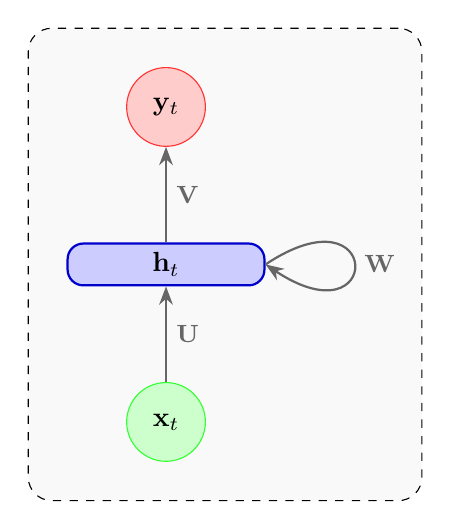
\begin{tikzpicture}[node distance=2cm, >=Stealth]

  % Main Box Container
  \node[main_box, minimum width=5cm, minimum height=6cm] (box) at (0.75,2.5) {};

  % Nodes using your styles
  \node[neuron_green] (x) at (0, 0.5) {$\mathbf{x}_t$};
  \node[plm_block] (h) at (0, 2.5) {$\mathbf{h}_t$};
  \node[neuron_red] (y) at (0, 4.5) {$\mathbf{y}_t$};

  % Vertical flow with weight labels
  \draw[arrow] (x) -- node[right, font=\small\bfseries] {$\mathbf{U}$} (h);
  \draw[arrow] (h) -- node[right, font=\small\bfseries] {$\mathbf{V}$} (y);

  % Recurrent Loop (The "Memory" aspect)
  % Using a loop to the side to show state feedback
  \draw[arrow] (h.east) .. controls +(1.5, 1) and +(1.5, -1) .. (h.east)
    node[midway, right, font=\small\bfseries] {$\mathbf{W}$};

  % Alternative feedback representation if you prefer the "delay" look
  % \draw[arrow] (h.west) -- ++(-1,0) -- ++(0,-1) -- ++(1,0) -- (h.west);

\end{tikzpicture}
\caption{The ``rolled'' representation of a RNN. Input \(\mathbf{x}_t\) is read for each time-step \(t\), multiplied by the input weight matrix \(\mathbf{U}\), the hidden state is updated using the hidden state weight matrix \(\mathbf{W}\), and the output is calculated using the updated hidden state and the output weight matrix \(\mathbf{V}\).}
\end{wrapfigure}

RNNs are a type of NN that are specifically designed to handle sequential data, particularly where data points depend on the context (points found earlier in the sequence). For example, a simple RNN known as an Elman Network \citep{elman_finding_1990}, the network maintains a hidden state \(\mathbf{h}\) as it reads each data point of an input one at a time. Each hidden state is calculated using the current input at time-step \(t\) and the previous hidden state:

\[\mathbf{h}_t = f_h(\mathbf{Ux} + \mathbf{Wh}_{t-1} + \mathbf{b}_h)\]

where \(f_h\) is the activation function, \(\mathbf{U}, \mathbf{W}\) are the learned weights for the input and hidden state, respectively, \(\mathbf{b}_h\) is the bias, and \(\mathbf{x}\) is the input. The output of the layer is calculated using the freshly updated hidden state:

\[\mathbf{y}_t = f_y(\mathbf{Vh}_t + \mathbf{b}_y)\]

where \(f_o\) is the activation function (not necessarily the same as the one for the hidden state), \(\mathbf{V}\) is the learned weights, and \(\mathbf{b}_y\) is the bias. RNNs suffer from the vanishing gradient problem, where the gradient shrinks rapidly over the time-steps, resulting in the ``forgetting'' of long-term dependencies. One architecture that addresses the vanishing gradient problem in RNNs is the LSTM \citep{lstm}, see Section \ref{LSTM_sec}.

\subsection{Long Short Term Memory}\label{LSTM_sec}

LSTMs are an extension of RNNs and are designed to combat the vanishing gradient problem. The intuition behind them is to use a learned mechanism to decide when the hidden state should be updated or reset, rather than continuously updating it at every time-step. This means that important information will be prioritized regardless of its position in the sequence of inputs.

This is achieved by adding an internal cell state governed by three ``gates'': the input gate, the forget gate, and the output gate. The internal cell state acts as the node's long-term memory. The input gate determines whether or not the current input and hidden state should affect the internal state. The forget gate determines whether or not the internal cell state should be reset (wiping the long-term memory). The output gate determines how much the internal cell state should affect the output (hidden state/short-term memory).

Each gate uses the logistic-sigmoid \(\sigma\) activation function, so the output is between \(0\) (let nothing through) and \(1\) (let everything through). The input \(\mathbf{i}_t\), forget \(\mathbf{f}_t\) and output \(\mathbf{o}_t\) gates are calculated by:

\[\mathbf{i}_t = \sigma(\mathbf{U}_i\mathbf{x}_t + \mathbf{W}_i\mathbf{h}_{t-1} + \mathbf{b}_i)\]
\[\mathbf{f}_t = \sigma(\mathbf{U}_f\mathbf{x}_t + \mathbf{W}_f\mathbf{h}_{t-1} + \mathbf{b}_f)\]
\[\mathbf{o}_t = \sigma(\mathbf{U}_o\mathbf{x}_t + \mathbf{W}_o\mathbf{h}_{t-1} + \mathbf{b}_o)\]

where \(\mathbf{U}\) and \(\mathbf{W}\) are weights, \(\mathbf{b}\) are the biases, \(\mathbf{x}\) is the input, and \(\mathbf{h}_{t-1}\) is the hidden state. Then, the internal cell state \(C_t\) is updated:

\[C_t = \mathbf{f}_t \odot C_{t-1} + \mathbf{i}_t \odot \tilde C_t\]

where \(\tilde C_t\) are the potential changes to the internal state, known as the input node, and calculated at time-step \(t\) with weights \(\mathbf{U}_c\) and \(\mathbf{W}_c\), and hidden state \(\mathbf{h}_{t-1}\):

\[\tilde C_t = \tanh(\mathbf{U}_c\mathbf{x}_t + \mathbf{W}_c\mathbf{h}_{t-1}+\mathbf{b}_c)\]

Finally, the hidden state is updated:

\[\mathbf{h}_t = \mathbf{o}_t \odot\tanh(C_t)\]

and both the hidden and internal states are used as input for the next time-step.

\subsubsection{Transformers}\label{Transformers}

\begin{wrapfigure}[30]{l}{7cm}
  
  \centering
  \resizebox{0.4\textwidth}{!}{
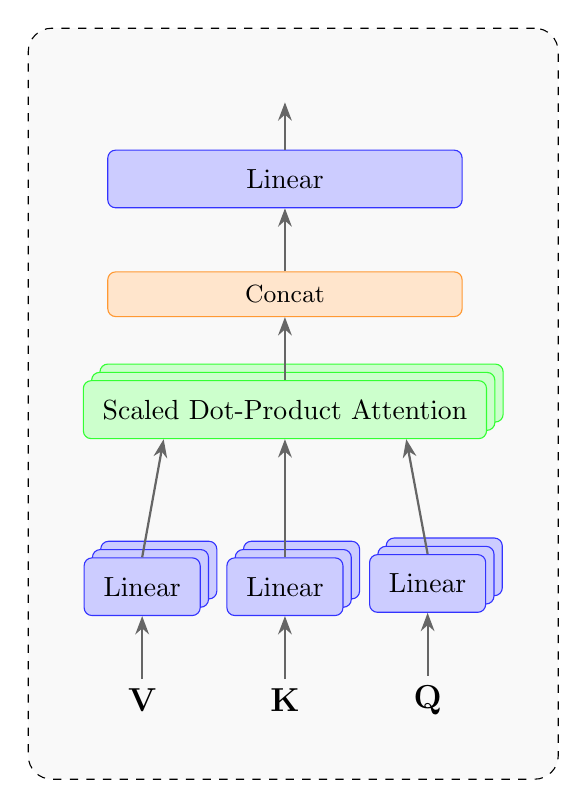
\begin{tikzpicture}[node distance=0.8cm]
\begin{scope}[local bounding box=attn]
    % Inputs
    \node (v) [input_node] {V};
    \node (k) [input_node, right=1.2cm of v] {K};
    \node (q) [input_node, right=1.2cm of k] {Q};

    \foreach \i in {v, k, q} {
        \node (l\i3) [parameters, above=0.8cm of \i, xshift=6pt, yshift=6pt] {Linear};
        \node (l\i2) [parameters, above=0.8cm of \i, xshift=3pt, yshift=3pt] {Linear};
        \node (l\i1) [parameters, above=0.8cm of \i] {Linear};
        \draw [arrow] (\i) -- (l\i1);
    }

    % Scaled Dot-Product Attention (using your latent_space style)
    \node (sdp3) [latent_space, above=1.5cm of lk1, xshift=6pt, yshift=6pt, minimum width=4.5cm] {Scaled Dot-Product Attention};
    \node (sdp2) [latent_space, above=1.5cm of lk1,  xshift=3pt, yshift=3pt, minimum width=4.5cm] {Scaled Dot-Product Attention};
    \node (sdp) [latent_space, above=1.5cm of lk1, minimum width=4.5cm] {Scaled Dot-Product Attention};
    \node (concat) [op_block, above=of sdp, minimum width=4.5cm] {Concat};
    \node (final)  [parameters, above=of concat, minimum width=4.5cm] {Linear};

    % Connections
    \draw [arrow] (lv1.north) -- ($(sdp.south west)!0.2!(sdp.south east)$);
    \draw [arrow] (lk1.north) -- (sdp.south);
    \draw [arrow] (lq1.north) -- ($(sdp.south west)!0.8!(sdp.south east)$);
    \draw [arrow] (sdp) -- (concat);
    \draw [arrow] (concat) -- (final);

    \node (out) [above=0.6cm of final] {};
    \draw [arrow] (final) -- (out);
  \end{scope}
\begin{scope}[on background layer]
          \node[main_box, fit=(attn.north west)(attn.north east)(attn.south east)(attn.south west)] (big_box) {};
      \end{scope} 
  \end{tikzpicture}}
  \caption{Multi-head attention module \citep{vaswani_attention_2017}. Each layer in the ``stack'' of linear projections projects the input with different weights, then passes them through the attention module, and finally concatenates them back together. The final linear projection returns the data to the original input dimension.}
\label{attention}
\end{wrapfigure}

The transformer architecture was introduced in 2017 by \citet{vaswani_attention_2017}, and quickly became the foundation for many state-of-the-art models in NLP like GPT \citep{radford_improving_2018} and BERT \citep{bert}. The transformer is based on an encoder-decoder structure, but with self-attention calculated in parallel via multiple ``heads''. Self-attention assigns weights to each token relative to each other, capturing important contextual information.

In the original transformer, attention is described as a mapping of queries, keys, and values to an output. The actual attention operation compares the queries and keys using dot product, then scaling, then softmax to determine the weights for each value. All queries, keys, and values are organized into their own matrices so that the attention can be computed on a set of queries simultaneously. The output is then just the weighted values:
\[\text{attention}(\mathbf{Q},\mathbf{K},\mathbf{V}) = \text{softmax}\left(\frac{\mathbf{QK}^\intercal}{\sqrt{d_k}}\right)\mathbf{V}\]

The original transformer uses multi-head attention, where the input of dimension \(d_m\) is a linearly projected concatenation of multiple attention ``heads'' whose queries, keys, and values are all projected with unique weight matrices to dimensions \(d_k, d_k, d_v\) respectively, allow the model to attend to different features simultaneously (see Figure \ref{attention}). More formally, multi-head attention can be defined as:

\[\text{multihead}(\mathbf{Q}, \mathbf{K}, \mathbf{V}) = \text{concat}(\text{head}_1, \dots, \text{head}_h)\mathbf{W^O}\] 

where \(\text{head}_i = \text{attention}(\mathbf{QW}_i^{\mathbf{Q}}, \mathbf{KW}_i^{\mathbf{K}}, \mathbf{VW}_i^{\mathbf{V}})\) with \(\mathbf{W}_i^{\mathbf{Q}} \in \mathbb{R}^{d_{m}\times d_k}, \mathbf{W}_i^{\mathbf{K}} \in \mathbb{R}^{d_{m}\times d_k}, \mathbf{W}_i^{\mathbf{V}} \in \mathbb{R}^{d_{m}\times d_v}\), and \(\mathbf{W^O} \in \mathbb{R}^{hd_{v}\times d_m}\).


\subsubsection{Variational Autoencoders}\label{VAE-sec}
A VAE combines the structure of a traditional autoencoder \citep{bank_autoencoders_2023} with variational inference and probabilistic modeling (Figure \ref{vae_architecture}). It is designed to translate the input into a distribution within its compressed, continuous, and structured internal representation known as the latent space, which allows it to generate new, similar data points through its decoder by sampling from the latent space and adding noise \citep{kingma_vae_2013}.

Assume the data generation process consists of sampling some latent vector \(\mathbf{z}\) from the latent distribution $p(\mathbf{z})$, then generating data \(\mathbf{x}\) from a conditional distribution $p_{\theta}(\mathbf{x}|\mathbf{z})$ parametrized by the decoder. To train the model we need to find the parameters $\theta$ that maximize the likelihood of \(\mathbf{x}\):

\[p(\mathbf{x}|\theta) = p_{\theta}(\mathbf{x}) = \displaystyle\int_{\mathbf{z}}^{}p_{\theta}(\mathbf{x}|\mathbf{z})p_{\theta}(\mathbf{z})d\mathbf{z}\] 

But this integral is intractable because it requires integrating over the large space of all $\mathbf{z}$. Since we can't compute $p_{\theta}(\mathbf{x})$, we can't compute the posterior $p_{\theta}(\mathbf{z}|\mathbf{x})$ either. Therefore, we introduce an approximate posterior parametrized by the encoder $q_{\phi}(\mathbf{z}|\mathbf{x})$. The loss function for training these networks (determining $\theta$ and $\phi$) is negative evidence lower bound (ELBO):

\[\mathcal{L}(\theta, \phi) = -\mathbb{E}_{q_{\phi}}[\log p_{\theta}(\mathbf{x}|\mathbf{z})] + D_{\text{KL}}[q_{\phi}(\mathbf{z}|\mathbf{x})||p(\mathbf{z})]\]

where $D_{\text{KL}}$ is the Kullback-Leibler (KL) Divergence. KL Divergence is a measure of the difference between two distributions \(p\) and \(q\). Specifically, it is the difference between cross-entropy and entropy:

\[D_{\text{KL}}(p(z)||q(z)) = \displaystyle\int\log\displaystyle\frac{p(z)}{q(z)}p(z)dz = \mathbb{E}_{p(z)}\left[\log\displaystyle\frac{p(z)}{q(z)}\right]\]

Some properties of KL Divergence are that, for all distributions \(p,q\) it is non-negative (\(D_{\text{KL}}(p||q) \ge 0\)), asymmetric (\(D_{KL}(p(z)||q(z)) \ne D_{\text{KL}}(q(z)||p(z))\)), equal to \(0\) if and only if \(p(z)\) and \(q(z)\) are equivalent, and does not satisfy the triangle inequality. Since KL Divergence is non-negative, \(\mathcal{L} \le p(x)\). \(p(x)\) is also called evidence, hence the name ELBO. 

Finally, the loss function involves random sampling, which makes backpropagation impossible. To avoid this, instead of outputting $\mathbf{z}$ directly, the encoder outputs the mean $\mu$ and variance $\sigma^2$ from which we can determine $\mathbf{z}$:
\[\mathbf{z} = \mu + \sigma \odot \epsilon\]
where $\epsilon$ is a random noise vector. With these modifications, the encoder and decoder can be optimized using gradient descent.

\begin{figure}
   \centering
   \begin{adjustbox}{width=\textwidth}
    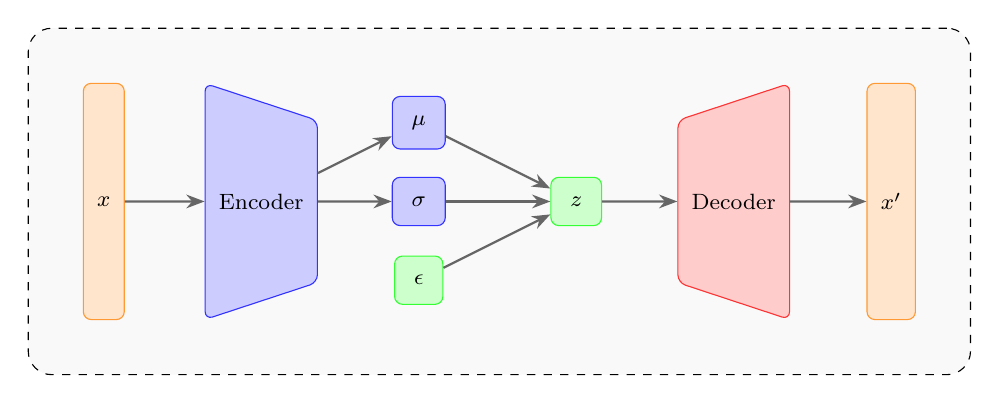
\begin{tikzpicture}

      \begin{scope}[local bounding box=vae]
        \node[encoder,font=\footnotesize](encoder) at (2,0) {Encoder};
        \node[decoder,font=\footnotesize](decoder) at (8,0) {Decoder};
        \node[vae_data,font=\footnotesize](input) at (0, 0) {\(x\)};
        \node[vae_data,font=\footnotesize](output) at (10,0) {\(x'\)};
        \node[parameters, font=\footnotesize](mean) at (4,1) {\(\mu\)};
        \node[parameters, font=\footnotesize](variance) at (4,0) {\(\sigma\)};
        \node[latent_space,font=\footnotesize](latent_space) at (6,0){\(z\)};
        \node[latent_space, font=\footnotesize](epsilon) at (4,-1){\(\epsilon\)};

        \draw[arrow] (input) -- (encoder);
        \draw[arrow] (decoder) -- (output);
        \draw[arrow] (encoder) -- (mean);
        \draw[arrow] (encoder) -- (variance);
        \draw[arrow] (mean) -- (latent_space);
        \draw[arrow] (variance) -- (latent_space);
        \draw[arrow] (epsilon) -- (latent_space);
        \draw[arrow] (latent_space) -- (decoder);
      
      \end{scope}
      \begin{scope}[on background layer]
          \node[main_box, fit=(vae.north west)(vae.north east)(vae.south east)(vae.south west)] (big_box) {};
      \end{scope} 
    \end{tikzpicture}
  \end{adjustbox}
  \caption{An illustration of the VAE architecture with the reparameterization trick for enabling backpropagation. Here, the encoder compresses the input \(x\) into \(\mu\) and \(\sigma\), which parameterize the latent space. \(z\) is sampled from that distribution using noise from \(\epsilon\), then passed as input to the decoder. The decoder attempts to recreate \(x\) as closely as possible.}
 \label{vae_architecture}
\end{figure}


\subsubsection{Generative Adversarial Networks}
A GAN is composed of two competing neural networks: a generator and a discriminator. They are trained simultaneously in an ``adversarial'' (or zero-sum game) process to generate new data that is indistinguishable from real data \citep{goodfellow2014generative}.

The generator $g_{\theta}(\mathbf{z})$ learns parameters $\theta$ to map a distribution $p(\mathbf{z})$ of noise to the data space $p(\mathbf{x})$. $g$ is trained to minimize $\log [1-d_{\phi}(g_{\theta}(\mathbf{z}))]$. Simultaneously, the discriminator $d_{\phi}(\mathbf{x})$ is trained to maximize the probability of correctly labeling real data $\mathbf{x}$ and generated data $g_{\theta}(\mathbf{z})$. The two models play the following minimax game with value function $v(g_{\theta}, d_{\phi})$:
\[\min_{g_{\theta}}\max_{d_{\phi}}v(g_{\theta}, d_{\phi}) = \mathbb{E}_{\mathbf{x}}[\log d_{\phi}(\mathbf{x})] + \mathbb{E}_{\mathbf{z}}[\log (1-d_{\phi}(g_{\theta}(\mathbf{z})))]\]
Where \(\mathbf{x}\) and \(\mathbf{z}\) are sampled from the training data and the noise distribution respectively. Both models are trained simultaneously to minimize and maximize the value function respectively via gradient descent.


\subsubsection{Diffusion Models}
Diffusion models learn to reconstruct data that was destroyed (typically by iteratively adding noise over time). Once the model is sufficiently trained, it can be given random noise to generate entirely new samples \citep{sohl-dickstein_deep_nodate}.

The destruction of the data is called the forward trajectory $q$, which adds noise to the original data $\mathbf{x}_0$ over $T$ time-steps until it is transformed into a simple prior distribution like the Gaussian. The joint probability of the forward process at each time-step is the product of the original data distribution and the transition (added noise) probabilities at each step:

\[q(\mathbf{x_0}, \mathbf{x_1}, \mathbf{x_2}, \ldots, \mathbf{x_T}) = q(\mathbf{x}_0)\prod_{t=1}^{T}q(\mathbf{x}_t|\mathbf{x}_{t-1})\]


\citet{sohl-dickstein_deep_nodate} used either a Gaussian diffusion kernel or a binomial diffusion kernel to model the transition $q(\mathbf{x}_t|\mathbf{x}_{t-1})$ for their experiments. 

The reconstruction of data from noise is called the reverse trajectory $p$, which reconstructs the original data $\mathbf{x}_0$ step-by-step from the simple prior $p(\mathbf{x}_T)$. The joint probability of the reverse process, similarly to the forward trajectory, is the product of the prior distribution and the reverse transition probabilities at each step:

\[p(\mathbf{x}_0, \mathbf{x}_1, \mathbf{x}_2, \ldots, \mathbf{x}_T) = p(\mathbf{x}_T)\prod_{t=1}^{T}p(\mathbf{x}_{t-1}|\mathbf{x}_t)\]

\citet{sohl-dickstein_deep_nodate}'s models learn to predict the mean and covariance of the kernel by minimizing the KL divergence of the forward and reverse trajectories. Modern diffusion models like \citet{ho_denoising_2020}'s DDPM predict the noise itself rather than the parameters of the noise's distribution. \citet{ho_denoising_2020} also simplifies the learning process by using mean square error (MSE) as the loss function, but the underlying theory remains the same. 

\section{Generative Models for PPI Prediction}
\begin{figure}[htbp]
  \centering
  \resizebox{\textwidth}{!}{
    \begin{forest}
      for tree={
        draw=blue!80,
        rounded corners,
        node options={align=center},
        fill=blue!20,
        edge={arrow}, % Ensure 'arrow' is defined in your \tikzset
        font=\sffamily,
        l sep=1cm,    
        s sep=0.5cm   
      }
      % Start the Tree
      [Literature Classification, 
        tikz+={
          \begin{scope}[on background layer]
            \node[main_box, fit=(current bounding box)] {};
          \end{scope}
        }
        [Model Type
          [LSTM
            [Sequence] [Structure] [Network]
          ]
          [Transformers
            [Sequence] [Structure]
          ]
          [VAEs
            [Structure] [Network]
          ]
          [GANs
            [Network]
          ]
          [Diffusion
            [Sequence]
          ]
        ]
      ]
    \end{forest}
  }
  \caption{The structure of how PPI prediction methods are classified in this review.}
  \label{classification_map}
\end{figure}


Generative models are effective at learning complex patterns in large datasets. When pre-trained on a protein-related learning task, a model learns useful information about the function of each amino acid and the shape of protein structures. This information is found as the activations in the model's hidden layers, and can be extracted to obtain a rich embedding. PPI prediction techniques use these embeddings as input into a trained classifier model for the final output.

There are three sources of data to be used for predicting PPIs: primary structure, tertiary structure (which contains primary and secondary structure inherently), and interaction networks. The first uses only the amino acid sequence of the proteins, the second uses the 3D shape of the protein, which inherently contains the sequence information, and the third uses a set of known PPIs to find new ones. Many network-based approaches also use primary structure. 

In this section, we classify each of the methods by the ML architecture of their model. Then, we further divide them by which protein features (sequence, structure, network) they use during training and deployment (see Figure \ref{classification_map}). It is notable that we did not find publications for every possible classification, and it is possible that some were missed.
\subsection{LSTMs}
Despite being introduced over 2 decades ago, LSTMs \citep{lstm} and their derivatives are still being developed \citep{beck_xlstm_2024}, and continue to be useful in the modern day. LSTM-based PLMs like UniRep \citep{alley_unified_2019} have recently been used to achieve high levels of accuracy in PPI prediction. UniRep \citep{alley_unified_2019} is a multiplicative long short-term memory (mLSTM) model trained on the UniRef50 \citep{suzek_uniref_2014} database to generate protein sequences. As the model processes a protein, the weights of the hidden layers are extracted for each amino acid position and averaged to give the output embedding.

\subsubsection{Sequence Based}
%TODO more detail
With a focus on human and virus PPIs, \citet{tsukiyama_lstm-phv_2021} proposed LSTM-PHV, a model that uses Word2Vec embeddings of amino acid k-mers as input into an LSTM, then classified using 4 fully connected layers. The model was trained on and uses sequence data.

\citet{dong_multitask_2021} proposed MTT, a model designed to identify human-virus PPIs that leverages the pre-trained UniRep. The embeddings are used as inputs for a single-layer perceptron that was fine-tuned on both human-human PPI prediction and human-virus PPI prediction to avoid overfitting on the smaller virus dataset. Multiplicative LSTMs like UniRep utilize an intermediate state \(\mathbf{m}_t\), which adds some scaling to the current input using the hidden state rather than only adding them for each gate \citep{krause2017multiplicativelstmsequencemodelling}. The following modifications are made to the traditional LSTM (see Section \ref{LSTM_sec}):

\[\mathbf{m}_t = (\mathbf{U}_m\mathbf{x}_t) \odot (\mathbf{W}_m\mathbf{h}_{t-1})\]
\[\mathbf{i}_t = \sigma(\mathbf{U}_i\mathbf{x} + \mathbf{W}_i\mathbf{m}_{t-1} + \mathbf{b}_i)\]
\[\mathbf{f}_t = \sigma(\mathbf{U}_f\mathbf{x} + \mathbf{W}_f\mathbf{m}_{t-1} + \mathbf{b}_f)\]
\[\mathbf{o}_t = \sigma(\mathbf{U}_o\mathbf{x} + \mathbf{W}_o\mathbf{m}_{t-1} + \mathbf{b}_o)\]
\[\tilde C_t = \tanh(\mathbf{U}_c\mathbf{x}_t + \mathbf{W}_c\mathbf{m}_{t-1}+\mathbf{b}_c)\]

\citet{sledzieski_d-script_2021} proposed D-SCRIPT, a sequence based model that leverages \citet{bepler_learning_2021}'s bi-directional LSTM (biLSTM) to generate embeddings. These pairs of embeddings are then used to compute a 2D contact map that encodes potential physical contact sites (potential interaction sites), which is used as input for the final pooling module that outputs the interaction probability. 

Bi-directional LSTMs utilize a second LSTM network that processes the input in the reverse order. The hidden state for the input \(x_t\) at time-step \(t\) is then a concatenation of both the forward network and backward network's hidden states:

\[\mathbf{h}_t = [\overrightarrow{\mathbf{h}}_t, \overleftarrow{\mathbf{h}}_t]\]

where \(\overrightarrow{\mathbf{h}}_t\) and \(\overleftarrow{\mathbf{h}}_t\) are the hidden states at time-step \(t\) for the forward and backward networks respectively. This allows the hidden states to learn both the ``past'' and ``future'' contexts of the sequence. 

RAPPPID was proposed by \citet{szymborski_rapppid_2022} and feeds each sequence through a two-layer bi-directional AWD-LSTM \citep{merity2017regularizingoptimizinglstmlanguage}, and then through a fully connected layer to obtain an embedding of each protein. Finally, the embeddings are concatenated and classified by a fully connected network.

\subsubsection{Network Based}
\citet{singh_topsy-turvy_2022} proposed Topsy-Turvy, a model that combines D-SCRIPT \citep{sledzieski_d-script_2021} and GLIDE \citep{devkota_glide_2020} to make use of both sequence and graph-based information to predict interactions. The model was designed to use graph information only during training, allowing the tool to be used with only sequence data as input.

\subsubsection{Structure Based}
A structure-aware extension of Topsy-Turvy, proposed by \citet{sledzieski_tt3d_2023}, incorporates structural data generated by Foldseek and AlphaFold 2 \citep{beck_xlstm_2024}. The embedding of the 3D structure is concatenated to the PLM embedding and trained with the same methodology as Topsy-Turvy. They aptly named the model Topsy-Turvy 3D (TT3D).

\subsection{Transformers}
The most common generative model based on the transformer for PPI prediction is ProtT5. ProtT5 is PLM based on Google's T5 architecture \citep{raffel_exploring_2020}. Its rich amino acid embeddings can be used not only for PPI prediction, but also for a diverse spread of bioinformatics problems like sequence alignment \citep{spicer_evaluating_2025}, protein classification \citep{shoombuatong_advancing_2025}, and a variety of prediction tasks \citep{schmirler_fine-tuning_2024}. Many of the recent state-of-the-art frameworks for PPI prediction make use of embeddings generated by ProtT5. Table \ref{tab:transformer_models_summary} shows each of the transformer-based models reviewed in this section, the type of protein data they use, and which PLM is used to generate the embeddings.

\begin{table}[ht]
    \centering
    \caption{Summary of transformer-based PPI Prediction Models, including data modalities and underlying PLMs.}
    \label{tab:transformer_models_summary}
    \begin{tabularx}{\textwidth}{@{} l l X l @{}}
        \toprule
        \textbf{Model} & \textbf{Reference} & \textbf{Data} & \textbf{PLM Embeddings} \\
        \midrule
        \text{xCAPT5} & \citet{dang_xcapt5_2024} & Sequence& ProtT5 \\
        \text{MaTPIP} & \citet{ghosh_matpip_2024} & Sequence + Manual Features & ProtT5 \\
        \text{ESM-PEFT} & \citet{sledzieski_democratizing_2024} & Sequence (PEFT) & ESM-2 \\
        \text{TUnA} & \citet{ko_tuna_2024} & Sequence (Uncertainty) & ESM-2 \\
        \text{ESM-AMP} & \citet{hosseini_c3pi_2025} & Sequence (Permutations) & ProtT5 \\
        \text{PLM-Interact} & \citet{liu_plm-interact_2025} & Sequence (Joint Enc.) & ESM-2 \\
        \text{ppIRIS} & \citet{piochi_ppiris_2025} & Sequence& ESM-2 \& ProstT5 \\
        \text{AttnSeq-PPI} & \citet{sarkar_attnseq-ppi_2026} & Sequence (Attention) & ProtT5 \\
        \text{SpatialPPIv2} & \citet{hu_spatialppiv2_2025} & Structure (GAT) & ProtT5 \\
        \text{DeepGNHV} & \citet{jiang_graph_2025} & Structure (AF2) & ProtT5 \\
        \bottomrule
    \end{tabularx}
\end{table}

\subsubsection{Sequence Based}
%NOTE xCAPT5
\citet{dang_xcapt5_2024} proposed xCAPT5, a model that leverages the embeddings generated by the ProtT5-XL-UniRef50 PLM \citep{elnaggar_prottrans_2022}, a multi-kernel deep convolutional siamese neural network, and the XGBoost algorithm. xCAPT5 predicts PPIs based solely on the primary structure. 

xCAPT5 takes the amino acid embeddings generated by ProtT5 and feeds them through individual CNNs with varying kernel sizes. The output of each kernel size is then pooled with average and max pooling, and concatenated to make a comprehensive representation of each protein. This process allows the model to retain information about local, fine-grained features as well as abstract global features simultaneously. 

The final representations of each protein are concatenated and used as input for an MLP with two densely connected layers. The internal representations of this MLP are fed into an XGBoost, which is trained to perform the final prediction. xCAPT5 attains state-of-the-art performance, but at the cost of model complexity. It also demonstrated that increasing the number of kernels can improve model performance for biological applications. 

%NOTE MaTPIP
\citet{ghosh_matpip_2024} proposed MaTPIP (Manual and pre-Trained PLM derived feature-based Protein-protein Interaction Predictor), a sequence-based approach to PPI prediction that fuses pre-trained PLM features with manually curated sequence attributes. In particular, it fuses the ProtT5-XL-UniRef50 model's embedding with position-specific scoring matrix (PSSM), LabelEncoding, SkipGram, BLOSUM62, autocovariance (AC), pseudo amino acid composition (PSEAAC), conjoint triad (CT), and local descriptor (LD), then uses a simple MLP to perform the final binary classification.

The authors found that the features obtained from ProtT5 were the most critical component of the model. They also note that the manually curated features contribute more in the scenario where the proteins in the test set appear in the training set, but with different interacting partners. They claim that this indicates that only the PLM features are not sufficient, and complementing them with manually curated features will result in better performance. 

%NOTE PEFT
Focusing on model efficiency, \citet{sledzieski_democratizing_2024} employed parameter-efficient fine-tuning on ESM-2 and fed the embeddings through an MLP for classification. However, they still achieved state-of-the-art on the \citep{bernett_cracking_2024} dataset, as one of the first to use it for training and testing. 

%NOTE TUNA 
Addressing the problem of model reliability, TUnA \citep{ko_tuna_2024} uses a spectral-normalized neural Gaussian process based on \citet{liu_simple_2020}'s paper to evaluate its uncertainty. ESM-2 protein embeddings and transformer-based encoders capture intra- and inter-protein features. Accounting for uncertainty in complex tasks can help reduce false positives and therefore the reliability of the model. Importantly, TUnA is one of the first models to be evaluated on \citet{bernett_cracking_2024}'s gold standard dataset and achieve performance better than random. 

Further exploring transformer-based contextual learning, ESM-AMP \citep{sun_esm2_amp_2025} uses ESM-2 embeddings to encode the pairs of proteins. Then, it passes the embeddings to a transformer encoder to learn the inter- and intra-protein interaction behaviour. Finally, an MLP is used for classification.

%NOTE C3PI
In order to incorporate some structural information from sequence data only, C3PI \citep{hosseini_c3pi_2025} randomly shuffles segments of the input proteins into 8 random permutations to expose the model to alternative orderings of the amino acids. The intuition is that doing this will allow residues that are distant in the sequence to be close to each other as they may be in the folded 3D structure of the protein. Each of these 8 random permutations is used as input for ProtT5, whose embeddings are combined and used for final classification. C3PI is another model that made use of \citet{bernett_cracking_2024}'s gold standard dataset.

%NOTE PLM-Interact
Rather than treating proteins as individual entities, PLM-Interact \citep{liu_plm-interact_2025} advocates for a ``joint encoding'' strategy. By concatenating both sequences before they enter a fully fine-tuned ESM-2 model, the architecture ensures that the embedding of each protein is intrinsically ``aware'' of the other throughout the network.


\citet{piochi_ppiris_2025} proposed ppIRIS, a model that uses both ESM-2 and ProstT5 (A fine-tuned version of ProtT5) to generate its embeddings. The embeddings are manipulated by siamese fully connected networks, concatenated, and passed through one final fully connected network for classification. Interestingly, the authors evaluated the model on the \citep{bernett_cracking_2024} gold standard, but did not report AUROC results, only accuracy, precision, recall, and f1.

The recently proposed AttnSeq-PPI \citep{sarkar_attnseq-ppi_2026} leverages ProtT5 embeddings to encode the proteins. The embeddings are then sent through a convolutional layer, and a custom self and cross attention module before being concatenated and classified by a feed-forward network. 

\subsubsection{Structure Based}
%NOTE SpatialPPIv2
\citet{hu_spatialppiv2_2025} proposed SpatialPPIv2, using both ProtT5 for sequence information embedding and graph attention networks (GATs) for 3D structural information embedding. Therefore, it uses both the primary and tertiary structure of the protein to inform its decisions.

When encoding tertiary structural data of proteins, each residue is represented as a node of a graph. The node contains information about the residue, the ProtT5 amino acid embedding in particular. An edge is added between two nodes if the distance between them in 3D space is below a certain threshold. An extra edge was added to connect each pair of residues between the two proteins to allow communication between them in the GAT. These edges are weighted according to their attention score, representing their corresponding amino acids' level of association. The learned features from the GAT are then used along with the ProtT5 embeddings, which are passed as input for a final fully connected classifier.

% NOTE DeepGNHV
DeepGNHV \citep{jiang_graph_2025} focuses on human-virus PPI prediction and uses a similar approach to \citet{hu_spatialppiv2_2025}. Much like SpacialPPIv2, DeepGNHV leverages ProtT5 for the sequence embeddings, but uses the artificial structure data generated by AlphaFold 2 \citep{jumper_highly_2021} due to the limited data available for human-virus PPIs. The architecture is also different. The embeddings from ProtT5 were not used as input directly into the final classifier, like SpatialPPIv2, but rather were only used for the nodes of the graph.

The general format of transformer-based PPI prediction models is as follows. First, use some pre-trained PLM to embed the protein sequences, whether it be joint (concatenated before embedding) or separate. Next, use the embeddings as input for some network, usually attention-based, to learn the relationship between the proteins. Finally, use a simple classifier network to output an interaction score or probability (see Figure \ref{fig:transformer-ppi}). Some models also embed the structural information of each protein. Mathematically, the interaction probability of the input pair of proteins can be defined as

\[p_{\text{interact}} = f_\theta(g_\theta(\text{concat}(\text{embeddings}, \text{structure}))\]

where

\[\text{embeddings} = \text{concat}(\text{plm}(\mathbf{a}), \text{plm}(\mathbf{b}))\]

for models that embed the sequences disjointly, or

\[\text{embeddings} = \text{plm}(\text{concat}(\mathbf{a}, \mathbf{b}))\]

for models that jointly embed the protein sequences \(\mathbf{a}\) and \(\mathbf{b}\) with strucural information encoded in \(\text{structure}\) (If structural information is not utilized, then this variable is empty and \(\text{concat}(\text{embeddings}, \text{structure}) = \text{embeddings}\)). The function \(f_\theta : \mathbb{R}^{d_z\times l}\rightarrow \mathbb{R}\) is a neural network (typically transformer based), parametrized by \(\theta\) that maps from the representation learning module's output space \(\mathbb{R}^{d_z\times l}\) to a real number representing the interaction score or probability, and the function \(g_\theta : \mathbb{R}^{d_e \times l}\rightarrow \mathbb{R}^{d_z\times l}\) is a network, parametrized by \(\theta\) that maps from the PLM embeddings to some latent space \(\mathbb{R}^{d_z\times l}\). Here, \(l\) is the combined length of the proteins, as PLMs like ProtT5 and ESM-2 output a vector for each amino acid in a sequence, \(d_z\) and \(d_e\) are the output dimensions of the representation learning module and the PLMs, respectively. Both \(f_\theta\) and \(g_\theta\) are typically trained simultaneously, hence the common parametrization. Note that this does not imply that the networks share weights.

\begin{figure}[htbp]
  \centering 
  \begin{adjustbox}{width=\textwidth}
    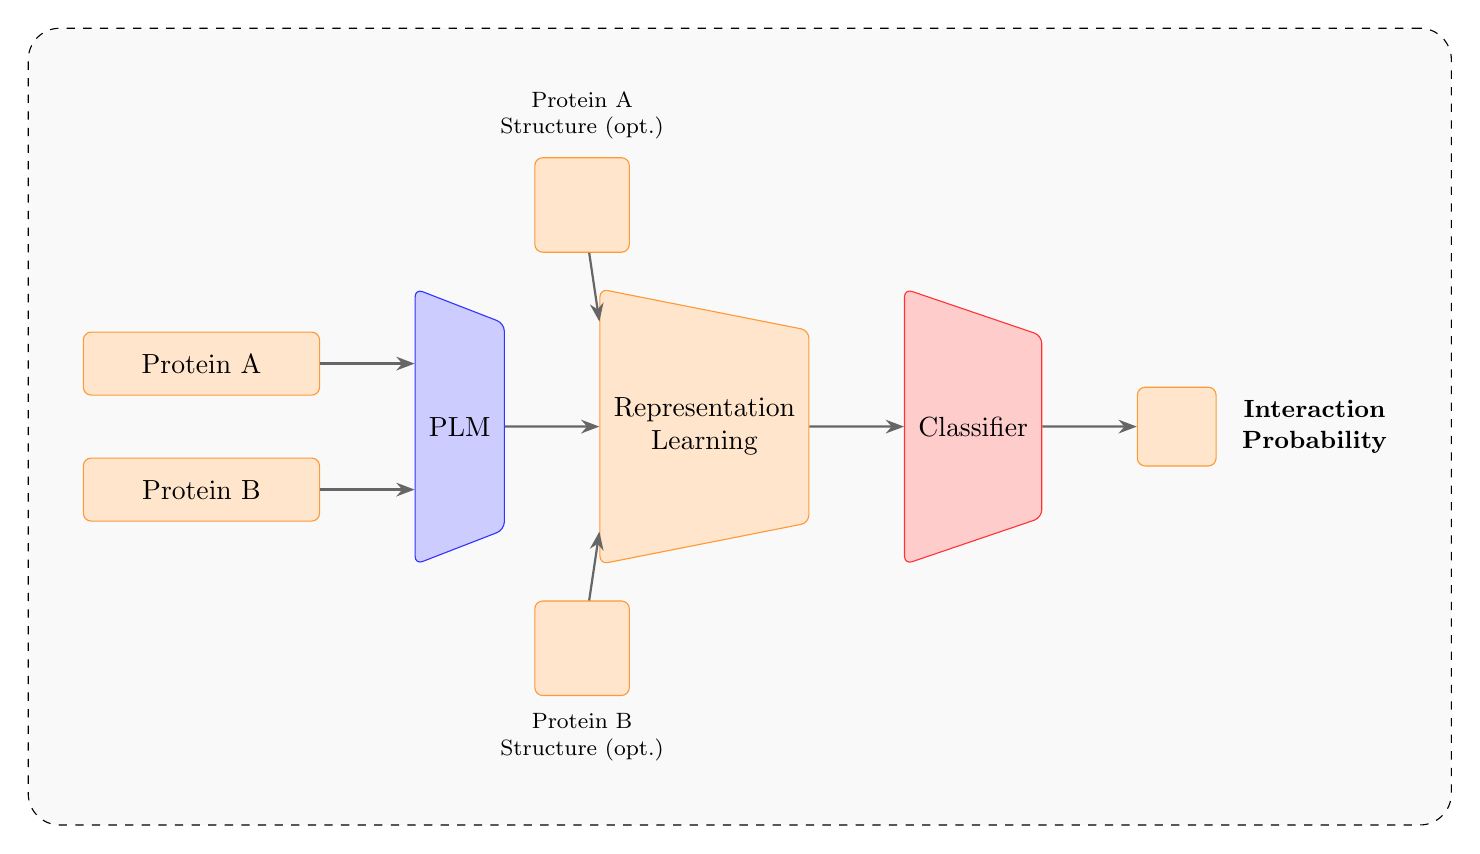
\begin{tikzpicture}[node distance=1cm and 1.5cm]
      \begin{scope}[local bounding box=box]
      
      % --- Main Blocks ---
      % Added 'align=center' to these nodes so '\\' works
      \node[encoder, minimum width=3.5cm, align=center] (plm) at (0,0) {PLM};
      
      \node[encoder, fill=orange!20, draw=orange!80, minimum width=3.5cm, right=1.2cm of plm, align=center] (features) {Representation\\Learning};
      
      \node[encoder, fill=red!20, draw=red!80, minimum width=3.5cm, right=1.2cm of features, align=center] (classifier) {Classifier};
      
      % --- Protein Inputs ---
      \node[vae_data, minimum width=3cm, minimum height=0.8cm, anchor=east] (protA) at ($(plm.west) + (-1.2, 0.8)$) {Protein A};
      \node[vae_data, minimum width=3cm, minimum height=0.8cm, anchor=east] (protB) at ($(plm.west) + (-1.2, -0.8)$) {Protein B};
      
      % --- Structure Inputs ---
      % Added 'align=center' to the label_text nodes as well
      \node[vae_data, minimum size=1.2cm] (structA) at ($(plm.north)!0.5!(features.north) + (0, 1.3)$) {};
      \node[label_text, above=0.1cm of structA, font=\footnotesize, align=center] {Protein A\\Structure (opt.)};
      
      \node[vae_data, minimum size=1.2cm] (structB) at ($(plm.south)!0.5!(features.south) + (0, -1.3)$) {};
      \node[label_text, below=0.1cm of structB, font=\footnotesize, align=center] {Protein B\\Structure (opt.)};

      % --- Output ---
      \node[vae_data, minimum size=1cm, right=1.2cm of classifier] (output) {};
      \node[label_text, right=0.2cm of output, align=center] {Interaction\\Probability};

      % --- Connections ---
      \draw[arrow] (protA) -- (protA -| plm.west);
      \draw[arrow] (protB) -- (protB -| plm.west);
      \draw[arrow] (plm) -- (features);
      \draw[arrow] (structA) -- (features.north west);
      \draw[arrow] (structB) -- (features.south west);
      \draw[arrow] (features) -- (classifier);
      \draw[arrow] (classifier) -- (output);
      \end{scope}

      % --- Background Box ---
      \begin{scope}[on background layer]
          \node[main_box, rounded corners=4mm, fit=(box)] (big_box) {};
      \end{scope} 
    \end{tikzpicture}
  \end{adjustbox}
  \caption{An illustration of the general structure of transformer-based PPI prediction models.}
  \label{fig:transformer-ppi}
\end{figure}

Some models, like xCAPT5 \citep{dang_xcapt5_2024}, keep the proteins separate until classification. Using the same notation as above, we can define this approach as:

\[p_{\text{interact}} = f_\theta(\text{concat}(g_\theta(\text{plm}(\mathbf{a}), \text{plm}(\mathbf{b}))))\] 

The functions \(f_\theta\) and \(g_\theta\) can be any form of NN. For example, in xCAPT5 \citep{dang_xcapt5_2024}, \(f_\theta\) is a MLP followed by XGBoost, and \(g_\theta\) is a series of CNNs. In TUnA \citep{ko_tuna_2024}, \(f_\theta\) is a spectral-normalized Gaussian process, and \(g_\theta\) is a custom transformer based module. In C3PI \citep{hosseini_c3pi_2025}, \(f_\theta\) is a MLP and \(g_\theta\) is their custom ``puzzler'' and ``entangler'' modules etc.

For structure-based methods, the data is encoded separately from the sequences and concatenated to the transformer embeddings. SpatialPPIv2 \citep{hu_spatialppiv2_2025} uses a GAT to encode the structural information of each protein and concatenates them all together prior to representation learning and classification.


\subsection{Variational Autoencoders}
\begin{table}[htbp]
    \centering
    \caption{Summary of VAE-based methods for PPI prediction.}
    \label{tab:vae_methods}
    \renewcommand{\arraystretch}{1.3} 
    % Reordered columns: Data Type (p), Model (l), Reference (l), Highlights (X)
    \begin{tabularx}{\textwidth}{@{} >{\raggedright\arraybackslash}p{2.5cm} l l X@{}}
        \toprule
        \textbf{Data} & \textbf{Model} & \textbf{Reference} & \textbf{Highlights} \\
        \midrule
        
        Sequence \& Structure & MAPE-PPI & \citet{wu_mape-ppi_2024} & Uses a VQ-VAE variant with a ``microenvironment codebook'' to encode primary and AlphaFold 2 tertiary structures. Trained via Masked Codebook Modeling. \\ 
        \addlinespace
        
        Sequence \& Structure & VQ-VAE & \citet{kiouri_structure-based_gut_2025} & Hybrid model fusing pre-trained VQ modules (from MAPE-PPI) with a bi-directional attention mechanism. Tailored for the human gut microbiome. \\
        \midrule
        
        Sequence \& Network & S-VGAE & \citet{yang_graph-based_2020} & Signed Variational Graph Auto Encoder using GCNs. Combines CT-extracted sequence features with local network topology to reconstruct the adjacency matrix. \\ 
        \addlinespace
        
        Network & HPIP & \citet{xiao_highly-confident_2021} & Partitions sparse PPIN matrices into blocks to train multiple VAEs. Sums output probabilities to predict high-confidence interactions in incomplete networks. \\
        
        \bottomrule
    \end{tabularx}
\end{table}

VAEs process information in a single pass, unlike RNNs, LSTMs, or transformers. This means that they must learn to represent the biological mechanisms and details of every amino acid in the protein, as well as their interactions with each other, all at once, and compress them into the latent space. This leads to serious loss of detailed information, and a focus on the ``big picture''. In sequence and structure-based PPI prediction, individual residue-level details are critical. Methods using VAEs are used as a complement to other architectures, or use interaction network information for their predictions. Table \ref{tab:vae_methods} provides a brief summary of VAE-based methods for PPI prediction.

\subsubsection{Structure Based}
%NOTE MAPE-PPI
\citet{wu_mape-ppi_2024} proposed MAPE-PPI, a model that uses a variant of a vector quantized variational autoencoder (VQ-VAE) to create a ``microenvironment codebook''. Using this codebook as a tool to encode proteins, a fully connected classifier network predicts the interaction type. MAPE-PPI uses the primary structure, and AlphaFold 2 predicted tertiary structure to predict interactions.

MAPE-PPI's microenvironment codebook was trained using masked codebook modeling (MCM) and by treating it as a learnable variable during the VQ-VAE training (no masking). Masked codebook modeling was inspired by masked language modeling from NLP, where certain tokens from the input are ``masked'' or ``corrupted'', and the model is tasked with predicting the missing tokens. The authors propose masking the codebook vectors directly rather than the input vectors and reconstructing the inputs based on the remaining codes. The intention of this is to avoid the possibility that random masking can lead to unwanted side effects \citep{pmlr-v162-shi22d, li_semmae_2022}. They linearly combine the loss from the unmasked task with the MCM task to be the total loss function used for training. MAPE-PPI outperformed other methods like PIPR \citep{chen_multifaceted_2019} and DPPI \citep{hashemifar_predicting_2018} on binary PPI prediction tests available at the time and provided a new representation learning model that generates high-quality protein embeddings.

%NOTE Derivative of MAPE-PPI
Training their model specifically for predicting PPIs in the human gut microbiome, \citet{kiouri_structure-based_gut_2025} proposed an architecture that uses concepts from VAEs and transformers. In particular, the pre-trained encoder and VQ modules from \citep{wu_mape-ppi_2024} are used to generate embeddings of each protein. These embeddings are then fused into a unified pair representation by a bi-directional attention module that uses an attention mechanism not dissimilar to the encoder of the original transformer, then concatenated and projected to obtain the final embedding. The final classification module is a series of fully connected layers that output a scalar interaction score.

\subsubsection{Network Based}
\citet{yang_graph-based_2020} proposed a framework for PPI prediction that incorporates sequence and interaction network information, leveraging their proposed variation of a VAE. The framework feeds the sequence information extracted by CT, and the local neighbourhood of the interaction network into a signed variational graph autoencoder (S-VGAE). The embeddings are extracted, and classified using a simple neural network.

The proposed S-VGAE uses graph convolutional networks (GCN) as the encoder. 
\[q(\mathbf{z}|\mathbf{x},\mathbf{A}) = \prod_\mathbf{z}\mathcal{N}(\mathbf{z}|\mu, \text{diag}(\sigma^2))\]
parametrized by GCNs: $\mu=\text{GCN}_{\mu}(\mathbf{x},\mathbf{A})$ and $\log\sigma = \text{GCN}_{\sigma}(\mathbf{x},\mathbf{A})$. The decoder tries to generate the adjacency matrix \(\mathbf{A}\) from the interaction network by assigning the logistic-sigmoid \(\sigma\) of the inner product of each pair of embeddings $\mathbf{z}_i$ and $\mathbf{z}_j$ as the interaction probability:
\[p(\mathbf{A}|\mathbf{z}) = \prod_{i=1}\prod_{j=1}p(\mathbf{A}_{ij}|\mathbf{z}_i, \mathbf{z}_j)\]
where
\[p(\mathbf{A}_{ij} = 1 | \mathbf{z}_i,\mathbf{z}_j) = \sigma(\mathbf{z}_i^T\mathbf{z}_j)\]

%NOTE HPIP
HPIP \citep{xiao_highly-confident_2021} is a VAE prediction model that predicts PPIs with a high level of confidence based on sparse (incomplete) protein-protein interaction networks (PPINs). HPIP partitions the matrix representation of the PPIN column-wise into 4 blocks, then generates 4 input matrices for 4 VAEs by selecting 3 of the partitions. Finally, summing the output probability matrices of each of the VAE-based predictors. The interactions are filtered to exclude known PPIs, and the remaining interactions with the highest probability sum are considered predicted, high-confidence interactions. HPIP fills out sparse PPINs with high-confidence predicted interactions. The authors argue that because the PPIN matrix is symmetric (PPINs are undirected graphs), blocking won't cause any information loss for each protein. They also argue that by parallelizing the workflow with multiple models, their architecture has potential for scaling. 



\subsection{Generative Adversarial Networks}

\begin{figure}[htbp]
  \centering 
  \begin{adjustbox}{width=\textwidth}
    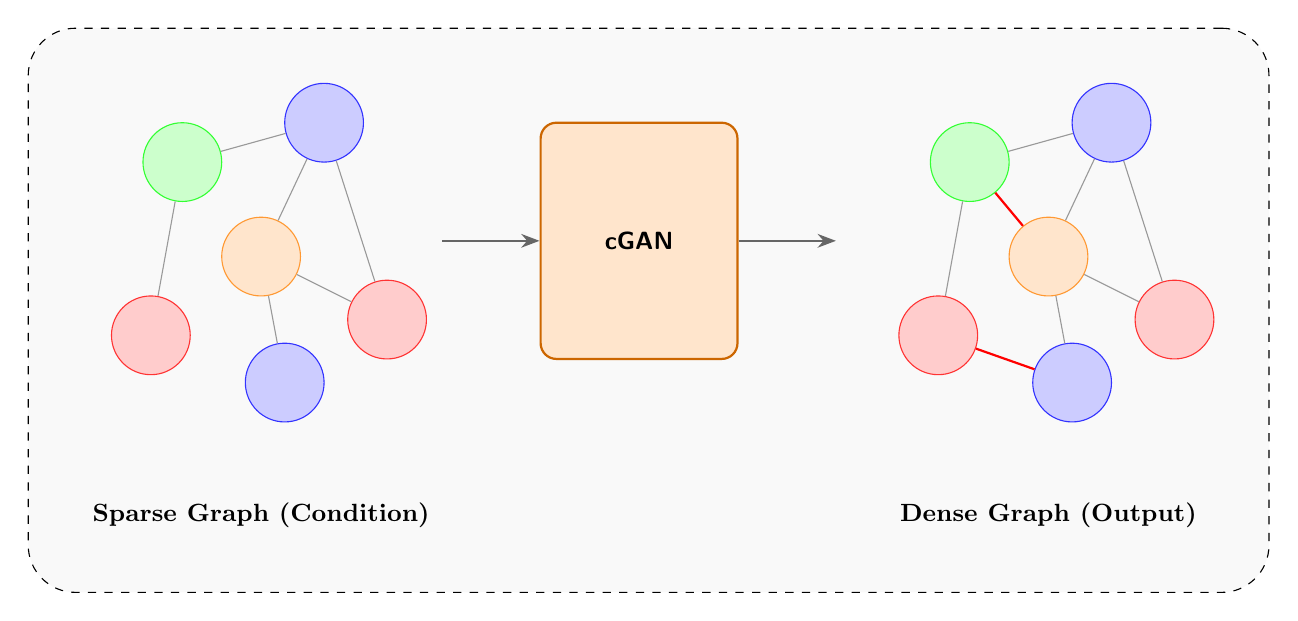
\begin{tikzpicture}
      \begin{scope}[local bounding box=box]
      % --- 1. Define Node Positions (Relative to a graph center) ---
      % We define these relative to (0,0) so we can copy them for Input and Output
      \def\graphNodes{
        % Top Right (Blue in ref)
        \node[neuron_blue] (n1) at (1, 1.5) {}; 
        % Top Left (Green in ref)
        \node[neuron_green] (n2) at (-0.8, 1) {};
        % Center (Yellow in ref)
        \node[neuron_yellow] (n3) at (0.2, -0.2) {};
        % Bottom Left (Pink in ref -> using Red)
        \node[neuron_red] (n4) at (-1.2, -1.2) {};
        % Bottom Center (Purple in ref -> using Blue)
        \node[neuron_blue] (n5) at (0.5, -1.8) {};
        % Bottom Right (Orange in ref -> using Yellow/Red)
        \node[neuron_red] (n6) at (1.8, -1.0) {};
      }

      % --- 2. INPUT GRAPH (Left) ---
      \begin{scope}[shift={(-5,0)}]
        \graphNodes % Draw nodes
        
        % Draw Edges matching your reference image
        \begin{pgfonlayer}{main}
          \draw[connect] (n4) -- (n2); % Pink - Green
          \draw[connect] (n2) -- (n1); % Green - Blue
          \draw[connect] (n1) -- (n3); % Blue - Yellow
          \draw[connect] (n1) -- (n6); % Blue - Orange
          \draw[connect] (n3) -- (n6); % Yellow - Orange
          \draw[connect] (n3) -- (n5); % Yellow - Purple
        \end{pgfonlayer}
        
        \node[label_text, below=2.5cm of n3] {Sparse Graph (Condition)};
        
        % Save coordinate for main arrow
        \coordinate (InputEdge) at (2.5, 0);
      \end{scope}


      % --- 3. cGAN PROCESS (Center) ---
      \node[process_block, minimum height=3cm, minimum width=2.5cm] (cgan) at (0,0) {cGAN};
    
      % --- 4. OUTPUT GRAPH (Right) ---
      \begin{scope}[shift={(5,0)}]
        \graphNodes % Draw exact same nodes
        
        % Draw ORIGINAL Edges (Gray)
        \begin{pgfonlayer}{main}
          \draw[connect] (n4) -- (n2);
          \draw[connect] (n2) -- (n1);
          \draw[connect] (n1) -- (n3);
          \draw[connect] (n1) -- (n6);
          \draw[connect] (n3) -- (n6);
          \draw[connect] (n3) -- (n5);
          
          % --- NEW EDGES (Red) ---
          % Adding just a couple edges to increase connectivity
          \draw[connect, draw=red, thick] (n2) -- (n3); % Green - Yellow
          \draw[connect, draw=red, thick] (n4) -- (n5); % Pink - Purple
        \end{pgfonlayer}
        
        \node[label_text, below=2.5cm of n3] {Dense Graph (Output)};
        
        % Save coordinate for main arrow
        \coordinate (OutputEdge) at (-2.5, 0);

      \end{scope}
      
      
      % --- 5. Main Flow Arrows ---
      \draw[arrow] (InputEdge) -- (cgan.west);
      \draw[arrow] (cgan.east) -- (OutputEdge);
\end{scope}
      \begin{scope}[on background layer]
          \node[main_box, rounded corners=6mm, fit=(box)] (big_box) {};
      \end{scope} 
    \end{tikzpicture}
  \end{adjustbox}
  \caption{\citet{balogh_efficient_2022}'s cGAN PPI link prediction model at inference. The incomplete graph is passed as the condition to the cGAN generator, which completes the graph.}
  \label{fig:cgan_graph}
\end{figure}

While GANs are effective at generating new examples of data, they do not explicitly learn the underlying distribution. This means that they are not required to learn a latent representation for proteins, and therefore cannot be used to generate embeddings. Without the ability to create embeddings of protein sequences or structures, they cannot be used for sequence or structure-based PPI prediction. However, this is not a problem for network-based methods since a GAN can be trained to generate an entire PPI network.

\subsubsection{Network Based}
\citet{balogh_efficient_2022} proposed a PPI network-based method for PPI prediction that uses a conditional generative adversarial network. The model is given lower connectivity subgraphs and trained to generate higher connectivity subgraphs (see Figure \ref{fig:cgan_graph}). This gives the model the ability to predict new links when testing on more complete networks. Most notably, it does not require any negative examples, as it does not directly classify individual pairs of proteins, but rather outputs an interaction score for every pair at once by generating a new, more connected adjacency matrix. Due to the clearly insufficient datasets of negative examples, avoiding the need for them is important. The alternative is supplementing the negative datasets with artificial negative samples from random pairs of proteins, which trains the classifier to learn the distinction between positive examples and unlabeled examples. Moreover, information about the proteins themselves was not used, only the interaction network, eliminating the dependence on external datasets. 

The model is based on the Pix2Pix architecture \citep{Isola_2017_CVPR}, modifying the discriminator to use a CNN in place of PatchGAN. The discriminator uses Wasserstein distance-based loss, causing it to act as a judge of the realism of the generator's output rather than classifying it as real or fake. This avoids cases of extreme imbalance where the discriminator learns at a much quicker rate than the generator, causing the gradient to vanish, or, on the other end, mode collapse. The authors note that their architecture is but one of many variations of the GAN model family, and that future research should investigate different architectures for both the generator and discriminator.

The interaction network is stored as an \(n\times n\) adjacency matrix \(\mathbf{M}^{n\times n}\), where \(n\) is the number of proteins in the network. During training, \(\mathbf{M}\) is thinned (some elements in \(\mathbf{M}\) are set to 0), and is passed to the cGAN generator to fill it back in. In this case, the discriminator tries to maximize the difference between its realism score for real pairs \((\mathbf{M},\mathbf{Y})\) and the generator (\(g_\theta\))'s pairs \((\mathbf{M}, g_\theta(\mathbf{M}, \mathbf{Z}))\). The generator's goal is to fool the discriminator and match the ground truth as closely as possible. This minimax game can be defined as:

\[\min_{g_\theta} \max_{d_\phi} \left( \mathbb{E}_{\mathbf{M}, \mathbf{Y}}[d_\phi(\mathbf{M}, \mathbf{Y})] - \mathbb{E}_{\mathbf{M}, \mathbf{Z}}[d_\phi(\mathbf{M}, g_\theta(\mathbf{M}, \mathbf{Z}))] \right) + \lambda \mathbb{E}_{\mathbf{M}, \mathbf{Y}, \mathbf{Z}}[\| \mathbf{Y} - g_\theta(\mathbf{M}, \mathbf{Z}) \|_1]\]

where \(\mathbf{M}\) is the condition (thinned adjacency matrix), \(\mathbf{Y}\) is the original adjacency matrix (ground truth), \(\mathbf{Z}\) is is the noise matrix, and \(\lambda\) is a hyperparameter for adjusting the weight of the reconstruction loss \(\mathbb{E}_{\mathbf{M}, \mathbf{Y}, \mathbf{Z}}[\| \mathbf{Y} - G(\mathbf{M}, \mathbf{Z}) \|_1]\).

\subsection{Diffusion Models}
Diffusion models recently started gaining popularity with the release of image generation models like DALL-E \citep{ramesh2021zeroshottexttoimagegeneration}, and more recently, text-to-video models like Sora \citep{videoworldsimulators2024}. Diffusion models have started to be applied to the PPI prediction problem, and other problems in bioinformatics like protein structure prediction \citep{abramson_accurate_2024}. 

\subsubsection{Sequence Based}
%NOTE DPLM
\citet{wang_diffusion_2024} proposed a diffusion protein language model (DPLM). DPLM is a discrete diffusion model based on recent work on diffusion like \citet{sohl-dickstein_deep_nodate}, \citet{hoogeboom2021argmaxflowsmultinomialdiffusion}, and \citet{austin2023structureddenoisingdiffusionmodels}. A discrete diffusion model uses a categorical (discrete) distribution to model the transition kernel \(q(\mathbf{x}_t|\mathbf{x}_{t-1})\) rather than a Gaussian or binomial continuous distribution.In particular, \citet{wang_diffusion_2024} define the forward transition kernel as 
\[q(\mathbf{x}_t|\mathbf{x}_{t-1}) = Cat(\mathbf{x}_t ; \beta_t\mathbf{x}_{t-1}+(1-\beta_t)\mathbf{q}_{noise})\]

where $\operatorname{Cat}(\mathbf{x}; \mathbf{p})$ is a categorical distribution on $\mathbf{x}$ 
parameterized by a vector $\mathbf{p}$, $\mathbf{q}_{\text{noise}}$ is the probability 
vector of the distribution $\operatorname{Cat}(\mathbf{x}_t; \mathbf{q}_{\text{noise}})$ 
(stationary distribution), and $0 < \beta_t < 1$ is a weight variable scheduling how much noise is added at each timestep. The reverse process is parameterized by 
a distribution that combines $q(\mathbf{x}_{t-1} | \mathbf{x}_t, \bar{\mathbf{x}}_0)$ 
with a distribution whose logits are predicted by a neural network 
$\bar{p}_{\theta}(\bar{\mathbf{x}}_0 | \mathbf{x}_t)$ summed over the one-hot 
representations of $\mathbf{x}_0$, $\bar{\mathbf{x}}_0$.

\[ p_{\theta}(\mathbf{x}_{t-1}|\mathbf{x}_t) = \sum_{\bar{\mathbf{x}}_0} q(\mathbf{x}_{t-1}, \mathbf{x}_t| \bar{\mathbf{x}}_0) \bar{p}_{\theta}(\bar{\mathbf{x}}_0|\mathbf{x}_t) \]

DPLM was tested on a multitude of both generative and discriminative downstream tasks, including PPI prediction. It outperformed ESM2 \citep{lin_evolutionary-scale_2023}, a popular PLM used for PPI prediction, on all tasks. \citet{wang_diffusion_2024} demonstrated that diffusion models for bioinformatics require further investigation.

%NOTE Failed Diffusion Model
\citet{quinn2025discriminativeproteinsequencemodelling} proposed the use of a denoising diffusion model operating on a protein autoencoder's latent space. The models' embeddings were evaluated on a variety of discriminative tasks, including PPI prediction, but did not perform at the level of masked language modeling or previous work on diffusion approaches \citep{wang_diffusion_2024}.

\section{Discussion}

\begin{table}
  \centering
  \caption{Model architecture and AUPR on \citet{bernett_cracking_2024}`s gold standard PPI dataset. ``*'' denotes results from \citet{bernett_cracking_2024}, otherwise results are from their paper of origin. ``---'' denotes models that have not been tested on the gold standard dataset.}
  \label{results}
  
  \begin{tabularx}{\textwidth}{l X X Z}
    \toprule
    \textbf{Model Type} & \textbf{Model} & \textbf{Reference} & \textbf{AUROC} \\ 
    \midrule
    \multirow{1}{*}{RNN} & *PIPR & \citet{chen_multifaceted_2019} & 0.532 \\
    \midrule
    \multirow{6}{*}{LSTM} & LSTM-PHV & \citet{tsukiyama_lstm-phv_2021} & --- \\ 
    & MTT & \citet{dong_multitask_2021} & --- \\ 
    & *D-SCRIPT & \citet{sledzieski_d-script_2021} & 0.499 \\ 
    & RAPPPID & \citet{szymborski_rapppid_2022} & --- \\
    & *Topsy-Turvy & \citet{singh_topsy-turvy_2022} & 0.587 \\ 
    & TT3D & \citet{sledzieski_tt3d_2023} & --- \\ 
    \midrule
    \multirow{10}{*}{Transformer} & xCAPT5 & \citet{dang_xcapt5_2024} & --- \\ 
    & MaTPIP & \citet{ghosh_matpip_2024} & --- \\ 
    & D-SCRIPT & \citet{sledzieski_democratizing_2024} & 0.690 \\ 
    & ESM\_AMP & \citet{sun_esm2_amp_2025} & 0.690 \\ 
    & TUnA & \citet{ko_tuna_2024} & 0.700 \\ 
    & C3PI & \citet{hosseini_c3pi_2025} & 0.703 \\ 
    & PLM-Interact & \citet{liu_plm-interact_2025} & 0.700 \\ 
    & ppIRIS & \citet{piochi_ppiris_2025} & --- \\ 
    & AttnSeq-PPI & \citet{sarkar_attnseq-ppi_2026} & 0.705 \\ 
    & SpacialPPIv2 & \citet{hu_spatialppiv2_2025} & --- \\ 
    & DeepGNVH & \citet{jiang_graph_2025} & --- \\ 
    \midrule
    \multirow{4}{*}{VAE} & MAPE-PPI & \citet{wu_mape-ppi_2024} & --- \\ 
    & Structure-based Gut & \citet{kiouri_structure-based_gut_2025} & --- \\ 
    & Graph-based & \citet{yang_graph-based_2020} & --- \\ 
    & HPIP & \citet{xiao_highly-confident_2021} & --- \\ 
    \midrule
    \multirow{1}{*}{GAN} & Efficient GAN & \citet{balogh_efficient_2022} & --- \\ 
    \midrule
    \multirow{2}{*}{Diffusion} & DPLM & \citet{wang_diffusion_2024} & --- \\ 
    & Denoising Diffusion & \citet{quinn2025discriminativeproteinsequencemodelling} & --- \\ 
    \bottomrule 
\end{tabularx}
\end{table}

\citet{jiang_graph_2025} showed that using predicted structures from algorithms like AlphaFold 2 can be useful for enhancing smaller datasets where tertiary structure data is not available. \citet{abramson_accurate_2024} introduced AlphaFold 3, a new iteration of AlphaFold that uses a transformer-based denoising (diffusion) model to generate accurate structures corresponding to sequences. Applying this latest innovation in protein structure prediction could boost performance and allow for high-quality extensions for smaller datasets.

While \citet{quinn2025discriminativeproteinsequencemodelling} and \citet{wang_diffusion_2024} were able to apply diffusion models to the problem of PPI prediction, there is still potential for future research in this area. A more sophisticated and rigorous fine-tuning approach on each of the classification tasks outlined in their papers, including PPI prediction, should be explored further.

Similarly, there has been little work applying adversarial networks to PPI prediction. \citet{balogh_efficient_2022} demonstrated that cGANs can be effectively used for this problem by leveraging interaction network information. Future research could investigate different approaches using primary or secondary structural information alongside the network information or explore different GAN variants.

On a more general note, models that train a separate classifier module must choose between having a limited number of true negative examples or artificially generating them. Both of these have drawbacks and are current limitations of the field. One solution to this is to avoid the need for negative examples during training at all, \citet{xiao_highly-confident_2021} and \citet{balogh_efficient_2022} employ this strategy. A method that leverages the power of generative AI to generate adjacency matrices to avoid the need for negative examples, while also making use of the rich information contained in the proteins themselves, is an interesting potential research avenue. Though the applicability of these models is questionable, since in the case that there is already an interaction graph for the interactome of interest, there is no reason to predict interactions. Models that memorize interaction network topology have been shown to have poor generalizability \citep{bernett_cracking_2024}.

Another general limitation is the lack of use of a high-quality, standardized test set. While \citet{bernett_cracking_2024} created such a dataset, it was released in 2024 and therefore has not yet been widely adopted (see Table \ref{results}). Most models have not been trained or evaluated on the new gold standard dataset. This means that some models that performed well may have success on the harder dataset, given that they are trained on it. Some future research could be to retrain the outdated models, as their poor performance could possibly be attributed to low-quality training data.

Of the models that were trained on \citet{bernett_cracking_2024}`s gold standard (\citet{sledzieski_democratizing_2024}, TUnA, C3PI, and PLM-Interact, etc., see Table \ref{results}), they perform similarly, but there is much room for improvement. It is apparent that the problem of PPI prediction is harder than initially thought, given the high and sometimes near-perfect performance reported on previous datasets. For all future research in this field, the \citet{bernett_cracking_2024} gold standard should be at least one of the datasets being used.

\section{Conclusion}
Recent advances in generative models have advanced the field of computational PPI prediction methods. In particular, they are capable of learning the complex underlying mechanisms of proteins, which can be leveraged to predict interactions at a high level of accuracy, though \citet{bernett_cracking_2024} demonstrated that most of these claimed accuracies are reliant on sequence similarity and node degree information.

Many recent models combine primary and tertiary structural data, or interaction network information, to enhance performance \citep{hu_spatialppiv2_2025, jiang_graph_2025, wu_mape-ppi_2024, kiouri_structure-based_gut_2025}. Some have even demonstrated that using artificially generated structures can still boost performance, especially on smaller datasets \citep{wu_mape-ppi_2024, jiang_graph_2025}.

In conclusion, generative models have advanced the state-of-the-art in PPI prediction, but remain plagued by inconsistent testing and unsatisfactory data. With the new Bernett dataset, this limitation may soon be overcome and could result in a faster, cheaper drug discovery process. 
%TODO Conclusion

% Bibliography
\bibliography{references}
\end{document}
